%%% Local Variables:
%%% mode: latex
%%% TeX-master: "../main"
%%% coding: utf-8
%%% End:
% !TEX TS-program = pdflatexmk
% !TEX encoding = UTF-8 Unicode
% !TEX root = ../main.tex

As discussed in the introduction and theory chapters, the goal of this work is to implement a web-based path tracer. The path tracer is designed to be used for product visualization based on engineering \gls{CAD} data, leveraging the \gls{OpenPBR} surface shading model and \gls{WebGPU}.

The concrete result of this work consists of multiple parts. The core is a path tracing library called \texttt{strahl}. The code and documentation are published under the \fGls{MIT license}{a permissive license originating at the Massachusetts Institute of Technology (MIT).} on GitHub, with an accompanying website. See \url{https://www.github.com/StuckiSimon/strahl} for details. This also includes detailed instructions on how to set up and configure the renderer. The library is published on the \fgls{npm}{a package manager for JavaScript.} registry as \texttt{strahl}. This report serves as the primary documentation of the work but does not contain library usage documentation. In addition, a dedicated short paper has been published for WEB3D '24: The 29th International ACM Conference on 3D Web Technology \cite{ownShortPaper}. The short paper includes the main insights and results of this work.

This chapter focuses on the implementation details and highlights design decisions of the path tracer. It also provides an overview of the available documentation, insights into the performance of the renderer, and its applicability for the described use case.

A consistent notation is used for references to the implementation of the path tracer. For example, \coderef{ABC} refers to the code with the same comment. All relevant places are marked in code using the same reference. This enables the use of search features to find the specific code section.

\section{Implementation}

The goal of the implementation is to be compatible with a large variety of devices and to make the setup for consumers straightforward. Therefore, it is implemented and tested mainly in Chrome, which uses \gls{Dawn} as the underlying implementation of \gls{WebGPU}. Most notably, this means that dedicated features from other implementations, such as \gls{wgpu}, cannot be used. Neither can experimental extensions be leveraged.

\autoref{fig:path-tracer} illustrates the procedure of the path tracer. Scene preparation is performed on the \gls{CPU}. This setup needs to be done once per visualization. Subsequent scene sampling is carried out repeatedly on the \gls{GPU}, which constitutes the most computationally intensive part of the process.

\begin{figure}[H]
    \includegraphics[width=1.0\columnwidth]{resources/path-tracer-pipeline.png}
    \caption{Path tracer pipeline, distinguishing \gls{GPU} and \gls{CPU} tasks. The stages of the compute pipeline and render pipeline are executed sequentially.}
    \label{fig:path-tracer}
\end{figure}

\subsection*{Scene Description}

In order to be easy to integrate for developers familiar with existing web-based rendering engines, the renderer utilizes many of the scene description constructs provided by \gls{Three.js}. This includes the representation of geometry using \texttt{BufferGeometry}, camera using \texttt{PerspectiveCamera}, and arbitrary camera controls such as \texttt{OrbitControls}. This also enables the use of a variety of loaders for different file formats, such as \gls{OBJ} or \gls{glTF}. However, due to its advantages for transmission, it's advised to use \gls{glTF}, which can be imported using the loader provided by \gls{Three.js}.

\subsubsection{Scene Preparation}

The primary process involved with setting up the scene is the preparation of the \gls{BVH}. For \gls{BVH} construction, well-established solutions for the web are available. The path tracer uses \texttt{three-mesh-bvh} \cite{threeMeshBvh}. This library builds the \gls{BVH} on the \gls{CPU} and is optimized for \gls{WebGL} use, which necessitates custom code for buffer creation in \gls{WebGPU}. See \coderef{BVH-TRANSFER} for transfer preparation.

In order to address memory alignment, as described in \autoref{ch:memoryAlignmentTheory}, the path tracer uses \texttt{webgpu-utils} \cite{webgpuUtilsLib}. The library enables a straightforward way to map data to buffers and align them correctly. See \coderef{MEMORY-VIEW} for the creation of the type definition and \coderef{BUFFER-MAPPING} for the mapping of data to buffers.

A high-level view of the data structures is shown in \autoref{fig:memory-structure}. Using the \gls{BVH}, it is possible to obtain the indices via indirect indices. Indirect indices are used because the \gls{BVH} re-orders them during construction. However, the original indices are needed to get the correct object definition, which stores the material information of the surface. See \coderef{BUFFER-BINDINGS} for the definition. \gls{WebGPU} enforces limits on the maximum number of storage buffers that can be employed per compute pipeline. Therefore, buffers for geometry data, which contain position and normal information per vertex, are interleaved in order to reduce the amount of storage buffers. Interleaving is the practice of putting multiple data types into the same buffer. The following sections will discuss more details on the specific buffer contents.

\begin{figure}[H]
    \centering
    \resizebox{1.0\textwidth}{!}{
        \tikzsetnextfilename{memory-structure}
        \begin{tikzpicture}[
                bvh/.style={rectangle, draw=rred, ultra thick, fill=rbred, inner sep=0.2cm, text width=3.0cm, align=center},
                geo/.style={rectangle, draw=rgreen, ultra thick, fill=rbgreen, inner sep=0.2cm, text width=3.0cm, align=center},
                mat/.style={rectangle, draw=rblue, ultra thick, fill=rbblue, inner sep=0.2cm, text width=3.0cm, align=center},
            ]

            \node[bvh] (bounds) {bounds};
            \node[bvh, above=0.6cm of bounds] (contents) {contents};

            \node[bvh, right=0.6cm of contents] (indirect) {indirect indices};
            \node[geo, right=0.6cm of indirect] (indices) {indices};

            \node[geo, right=0.6cm of indices] (geometry) {geometry};

            \node[mat, below=0.6cm of indices] (object) {object definitions};
            \node[mat, right=0.6cm of object] (materials) {materials};

            \draw[thick] (bounds) -- node[midway, right] {1:1} (contents);
            \draw[-latex, thick] (contents) -- (indirect);
            \draw[-latex, thick] (indirect) -- (indices);
            \draw[-latex, thick] (indices) -- (geometry);
            \draw[-latex, thick] (indices) -- (object);
            \draw[-latex, thick] (object) -- (materials);
        \end{tikzpicture}}
    \caption{Main data buffers used by the path tracer. Data structures associated with the \gls{BVH} are red, geometry information is green, and material or object information is blue. Arrows indicate the pointers between the buffers.}
    \label{fig:memory-structure}
\end{figure}

\subsection*{Ray Generator}

The ray generator is responsible for casting rays into the scene according to the view projection. For parallelization, each ray is cast in a separate thread; the degree of possible parallelization depends on the image's resolution. The path tracer employs a backward ray tracing approach, tracing rays from the camera into the scene. For many applications, especially photorealistic rendering, perspective projection is prevalent. Therefore, based on the assessed use case, the path tracer uses perspective projection. See \coderef{VIEWPROJECTION} for implementation.

\label{sec:anti-aliasing-implementation}

For \gls{RNG}, the path tracer uses \gls{PCG}, specifically the \texttt{PCG-RXS-M-XS} variant, as described by O’Neill \cite{o2014pcg}. See \coderef{RNG} for implementation. In order to set up the Monte Carlo sampling, the \gls{RNG} needs to be employed in a suitable manner. As a pseudorandom generator, \gls{PCG} necessitates a seed to start the cycle. If the seed is identical for all pixels, the results of a single sample will frequently share similar patterns in adjacent surfaces, as shown in \autoref{fig:rngBadSeed}. The result for independent seeds differs in a pronounced manner, as demonstrated in \autoref{fig:rngGoodSeed}.

\begin{figure}[H]
    \centering
    \begin{subfigure}[b]{0.45\textwidth}
        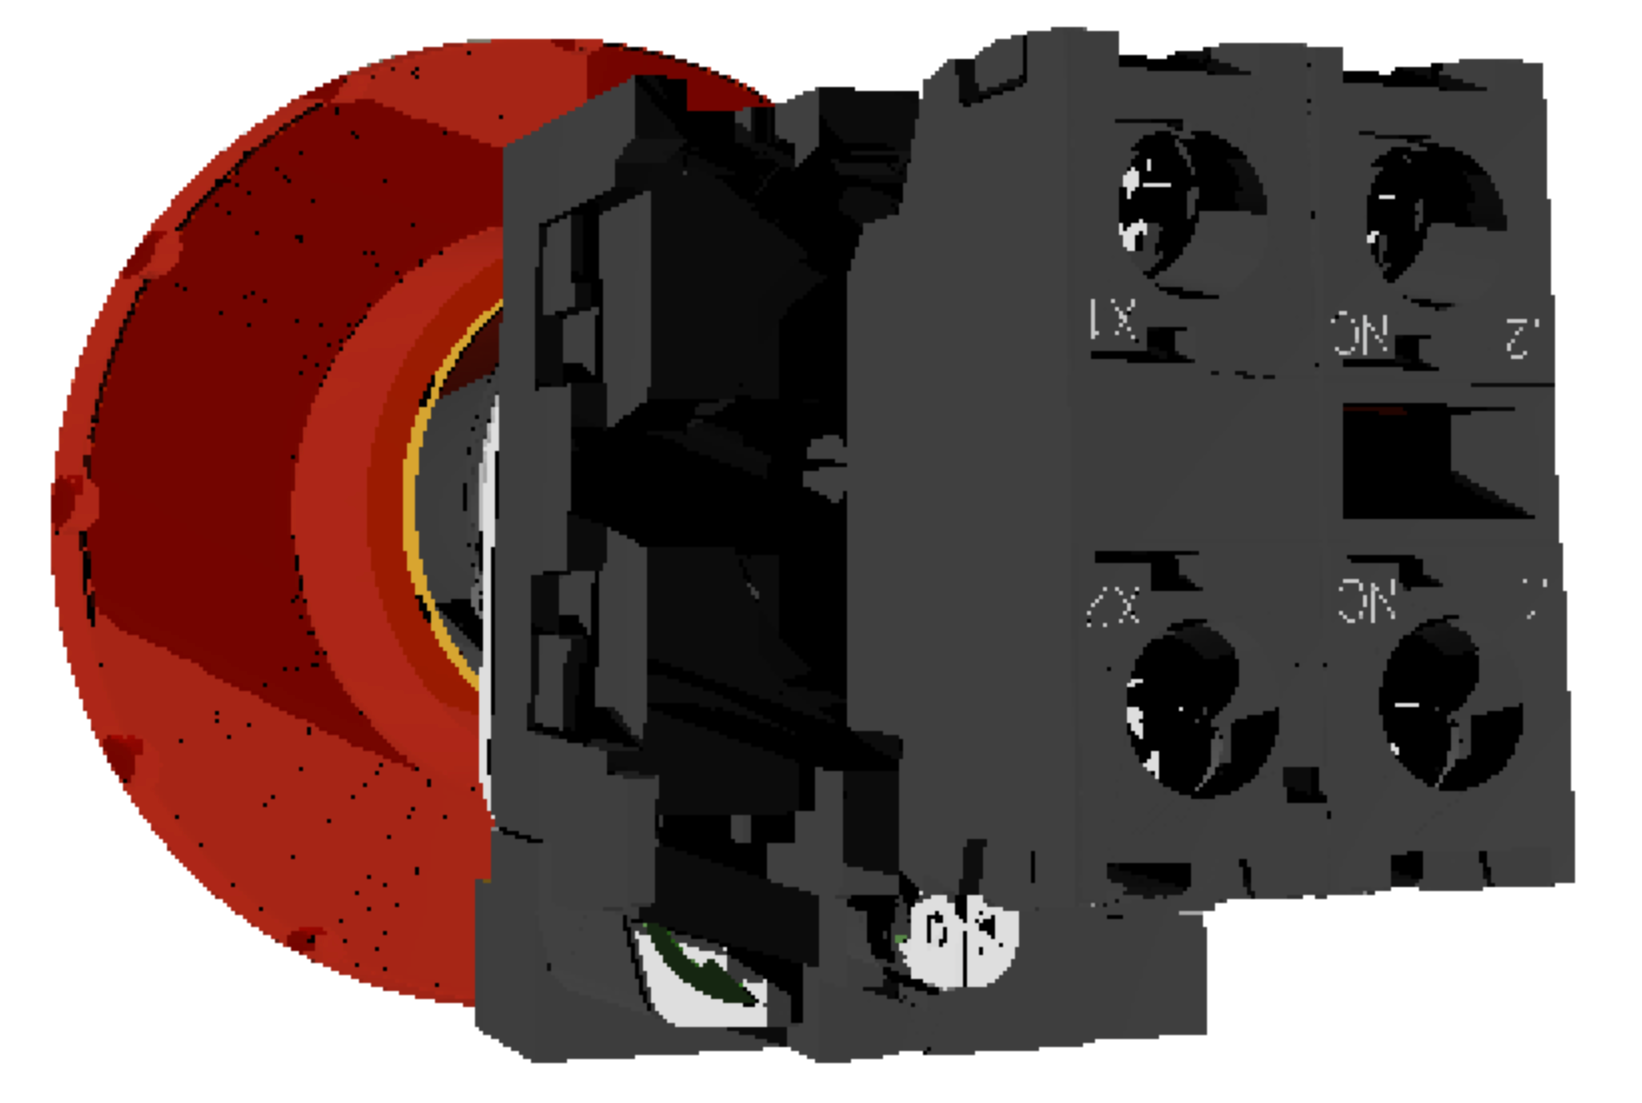
\includegraphics[width=\textwidth]{resources/single-sample-bad-seed.png}
        \caption{Identical seed for all pixels.}
        \label{fig:rngBadSeed}
    \end{subfigure}
    \hfill
    \begin{subfigure}[b]{0.45\textwidth}
        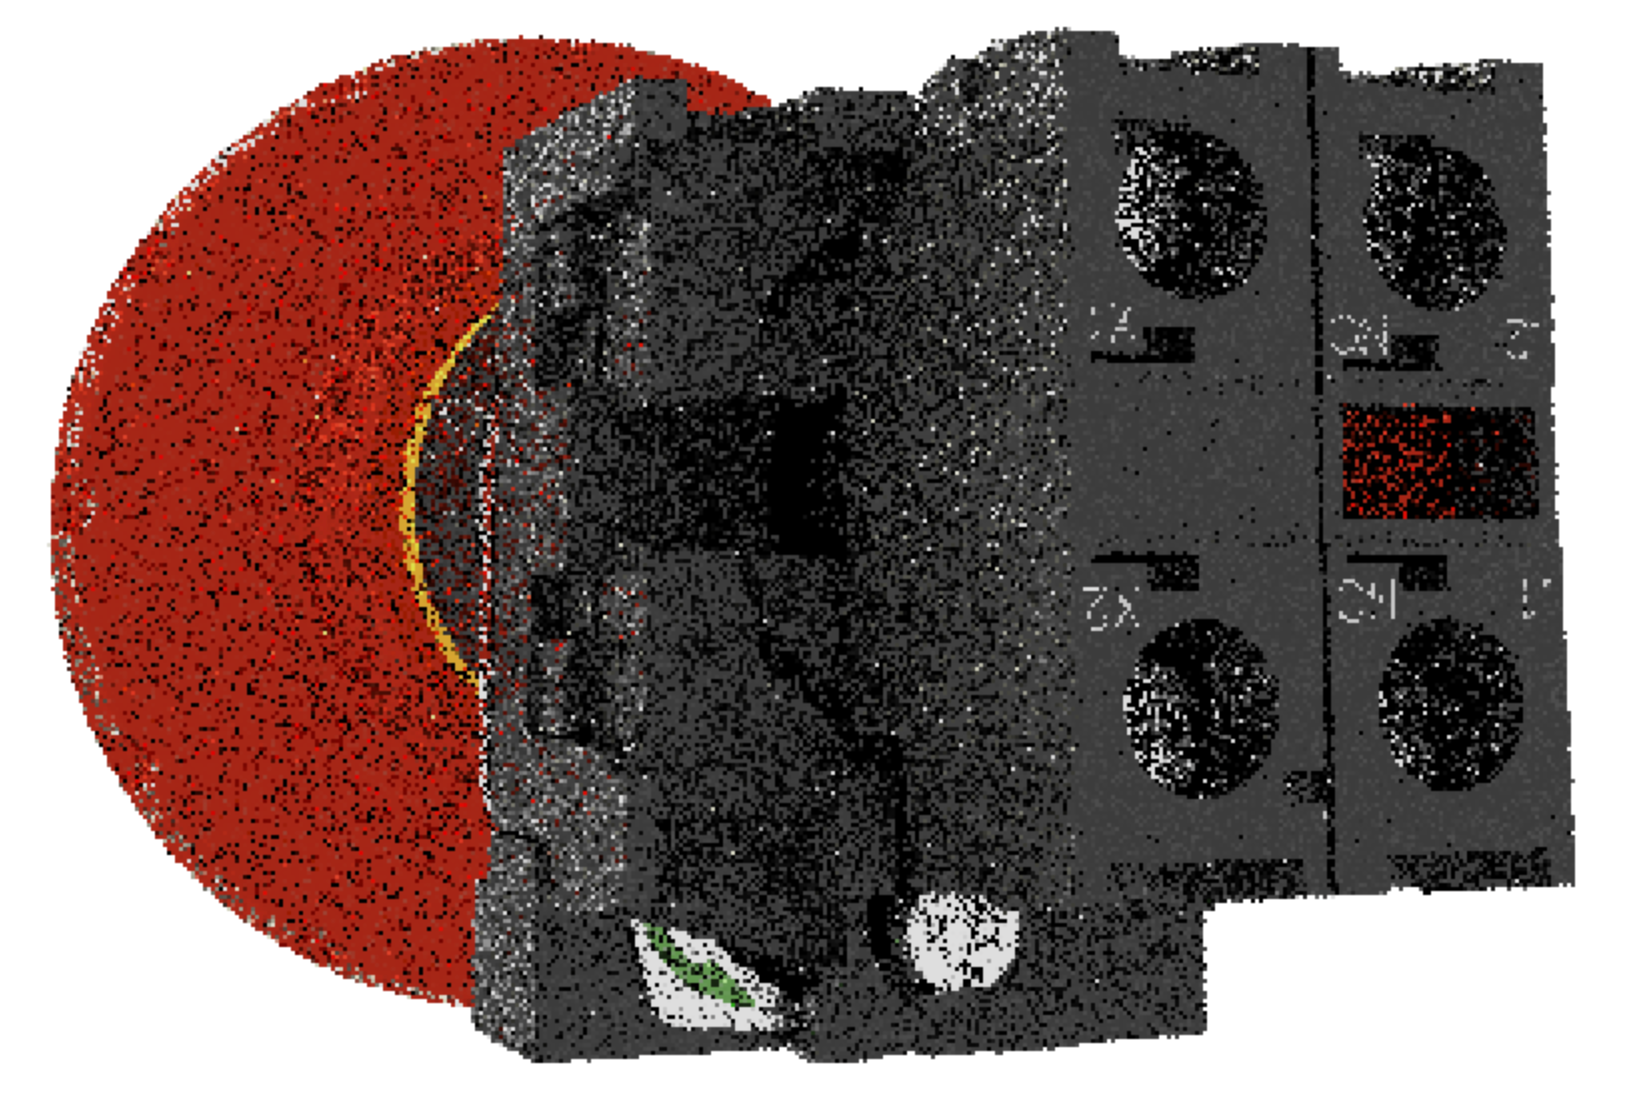
\includegraphics[width=\textwidth]{resources/single-sample-good-seed.png}
        \caption{Independent seed for every pixel.}
        \label{fig:rngGoodSeed}
    \end{subfigure}
    \caption{Both images consist of only one sample.}
    \label{fig:rngSeed}
\end{figure}

When increasing the sample count, the differences in the setup remain visible. Adjacent surfaces show similar patterns, as shown in \autoref{fig:rngNoiseArtifactsHighlightsBadNoisy}. These patterns resemble image compression artifacts encountered in aggressively compressed \fGlspl{JPEG}{\e{Joint Photographic Experts Group}, a common method for lossy image compression.}. In contrast, the renderings with independent seeds show stark differences in adjacent pixels akin to noise, as shown in \autoref{fig:rngNoiseArtifactsHighlightsGoodNoisy}. As shown in \autoref{fig:rngNoiseArtifactsHighlightsBadAnti} compared to \autoref{fig:rngNoiseArtifactsHighlightsGoodAnti}, the anti-aliasing is less noticeable when using independent seeds. The implementation of the anti-aliasing strategy indicated in \autoref{sec:anti-aliasing} is implemented in \coderef{ALIASING} and is highly dependent on the \gls{RNG} setup.

\begin{figure}[H]
    \centering
    \hspace*{2cm}
    \begin{subfigure}[t]{0.3\textwidth}
        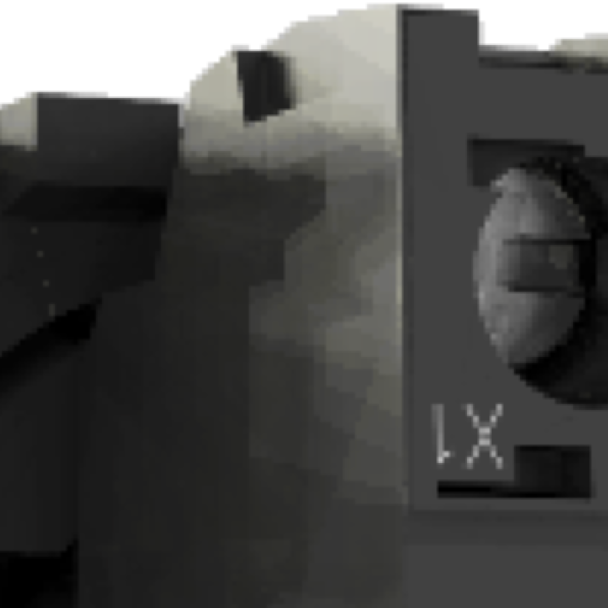
\includegraphics[width=\textwidth]{resources/bad-seed-noisy.png}
        \caption{Renderings which resemble lossy image compression artifacts.}
        \label{fig:rngNoiseArtifactsHighlightsBadNoisy}
    \end{subfigure}
    \hfill
    \begin{subfigure}[t]{0.3\textwidth}
        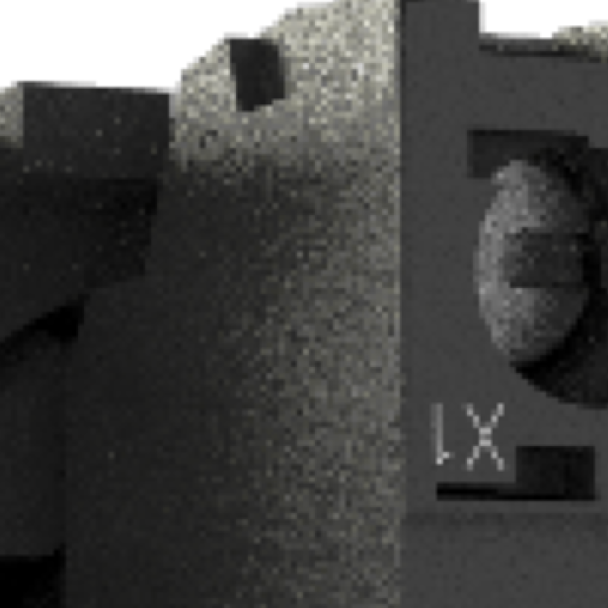
\includegraphics[width=\textwidth]{resources/good-seed-noisy.png}
        \caption{Noisy renderings with stark differences in adjacent pixels.}
        \label{fig:rngNoiseArtifactsHighlightsGoodNoisy}
    \end{subfigure}
    \hspace*{2cm}
    \vfill
    \vspace*{0.5cm}
    \hspace*{2cm}
    \begin{subfigure}[t]{0.3\textwidth}
        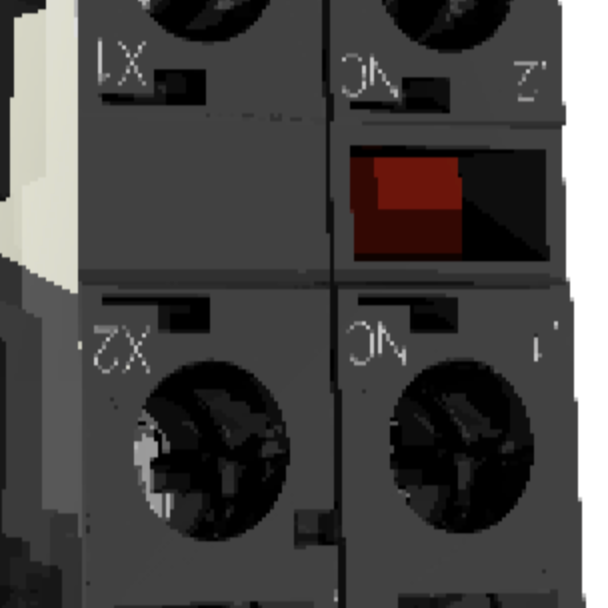
\includegraphics[width=\textwidth]{resources/bad-seed-anti-aliasing.png}
        \caption{On the right side of the image, anti-aliasing is rather noticeable.}
        \label{fig:rngNoiseArtifactsHighlightsBadAnti}
    \end{subfigure}
    \hfill
    \begin{subfigure}[t]{0.3\textwidth}
        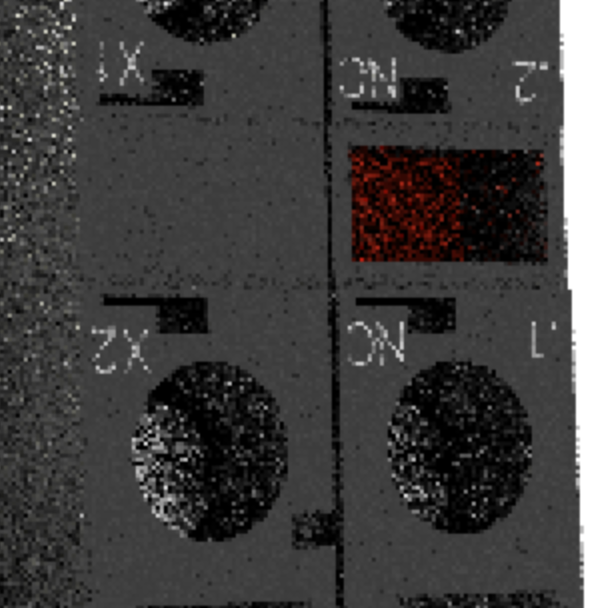
\includegraphics[width=\textwidth]{resources/good-seed-anti-aliasing.png}
        \caption{On the right side of the image, anti-aliasing is less noticeable.}
        \label{fig:rngNoiseArtifactsHighlightsGoodAnti}
    \end{subfigure}
    \hspace*{2cm}
    \caption{Magnified images of renderings with low sample count showing differences based on seed setup. The left column has an identical seed for all pixels of a sample but varying seeds for different samples. The right column has independent seeds for every pixel of a sample as well as across samples.}
    \label{fig:rngNoiseArtifactsHighlights}
\end{figure}

\subsection*{Path Tracer}

The path tracer is the core of the library and is responsible for intersection testing, conducting scene sampling, and calculating the final radiance. The basic procedure can be seen in \autoref{fig:path-tracer-workflow}. The ray, cast by the ray generator, is tested for intersections. If it misses, the path will be terminated. If a surface hit is detected, the shading will be generated based on the \gls{OpenPBR} specification. The shading generates a new scattered ray and determines the throughput of the ray. Russian roulette uses the throughput to perform probabilistic path termination. If it should be continued, the ray is cast again. The max depth of the ray determines the end of the path. During termination, the radiance contribution is collected in \fGls{RGB}{\e{red, green, and blue}, a common system for color representation in computer graphics.} color space.

\begin{figure}[H]
    \centering
    \tikzsetnextfilename{path-tracer-workflow}
    \begin{tikzpicture}[
            pre/.style={rectangle, draw=lightgray, ultra thick, inner sep=0.2cm, text width=3.0cm, align=center},
            core/.style={rectangle, draw=rblue, ultra thick, fill=rbblue, inner sep=0.2cm, text width=3.0cm, align=center},
        ]

        \node[pre] (ray) {Ray Generator};
        \node[core, right=1.5cm of ray] (intersection) {Intersection Test};
        \node[core, below left=1.2cm and 0cm of intersection] (shader) {Surface Shading};
        \node[core, right= 3cm of shader] (russian) {Russian Roulette};
        \node[pre, right= 1.5cm of intersection] (terminate) {Termination};

        \draw[-latex, thick] (ray) -- node[midway, above] {ray} (intersection);
        \draw[-latex, thick] (intersection) -- node[midway, left=0.2cm] {surface} (shader);
        \draw[-latex, thick] (shader) -- node[midway, above] {throughput} node[midway, below] {ray} (russian);
        \draw[-latex, thick] (intersection) -- (terminate);
        \draw[-latex, thick] (russian) -- (terminate);
        \draw[-latex, thick] (russian) -- node[midway, right] {ray} (intersection);
    \end{tikzpicture}
    \caption{High-level workflow of core path tracing routine. Blue are the main parts of the recursive path tracing algorithm, gray are the pre- and post-processing steps. The arrows indicate the flow of data, describing the primary information passed between the steps.}
    \label{fig:path-tracer-workflow}
\end{figure}

\subsubsection{Intersection Test}
\label{sec:bvh-implementation}

Intersection tests based on the \gls{BVH} are implemented in \gls{WGSL}, see \coderef{BVH-TESTS} for details. The intersection tests for triangles are implemented in \coderef{TRIANGLE-INTERSECTION}. The boundary data is stored as \gls{AABB} requiring two vectors for the minimum and maximum bounds. The \gls{BVH} node content depends on whether it is a leaf or an inner node. Each node uses 64 bytes of memory, as visualized in \autoref{fig:bvh-info}. The split axis determines which child node is traversed first. The left index is the index of the sibling node. Therefore, only the right index is stored. For leaf nodes, the triangle offset determines the index in the indirect indices buffer. The triangle count is the number of triangles in the leaf node.

\begin{figure}[H]
    \centering
    \begin{subfigure}[b]{0.45\textwidth}
        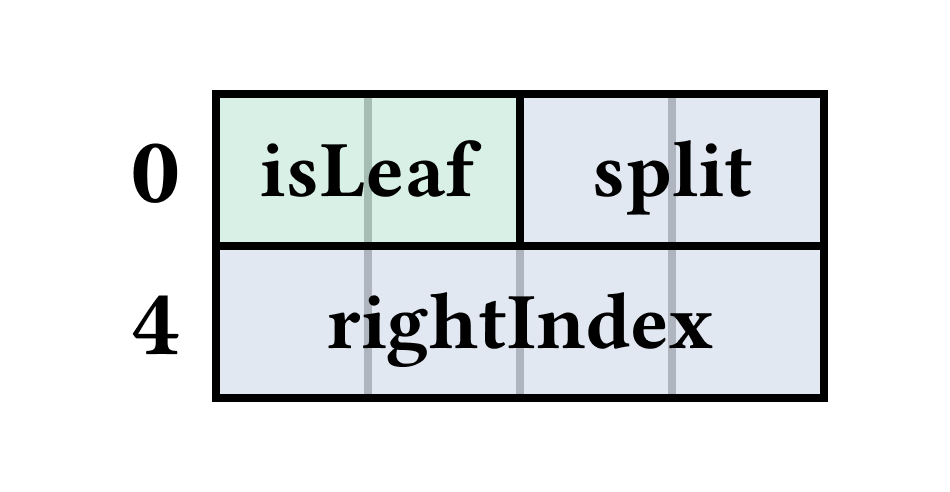
\includegraphics[width=\textwidth]{resources/bvh-node-info.png}
        \caption{\gls{BVH} inner node information.}
        \label{fig:bvh-info-inner-node}
    \end{subfigure}
    \hfill
    \begin{subfigure}[b]{0.45\textwidth}
        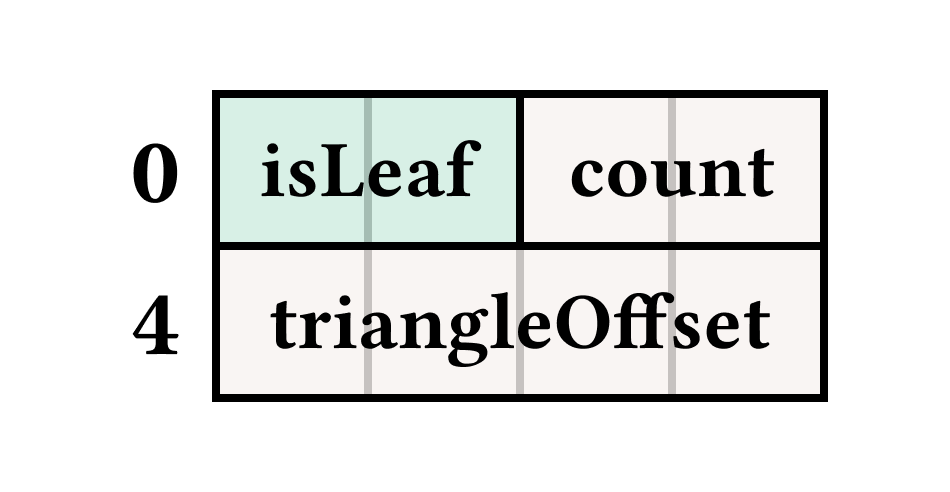
\includegraphics[width=\textwidth]{resources/bvh-leaf-info.png}
        \caption{\gls{BVH} leaf node information.}
        \label{fig:bvh-info-leaf-node}
    \end{subfigure}
    \caption{Content information stored in \gls{BVH} nodes. The information in the first two bytes is used to discriminate between inner and leaf nodes.}
    \label{fig:bvh-info}
\end{figure}

\subsubsection{Surface Shading}

For each intersection, sampling is done according to the \gls{MIS} scheme using a combination of light source sampling and \gls{BSDF} sampling as described in \autoref{sec:monte-carlo-integration-sampling}. For light source sampling, an additional shadow ray is cast to determine the visibility of the light source. See \coderef{RAY-COLOR} for implementation. The surface shading method is based on the \gls{OpenPBR} reference implementation in \gls{MaterialX} and the reference viewer by Portsmouth \cite{openPbrViewer}. Shading starts by sampling the reflection functions based on definitions of \gls{OpenPBR}, which reference the Monte Carlo sampling scheme described in the \gls{pbrt} book \cite{Pharr_Physically_Based_Rendering_2023} for sampling \glspl{BSDF}, as described in \autoref{sec:bxdf}. See \coderef{REFLECTION-LOBE-WEIGHTS} and subsequent methods for implementation. Using these probabilities, one specific reflection lobe is sampled, and an outgoing direction is determined as implemented in \coderef{BSDF-SAMPLE}. These different lobes correspond to different workflows, such as diffuse, specular, or metal. The implementation does not constitute a complete conformance to the \gls{OpenPBR} specification but instead covers a subset of the features.

The outgoing path and radiance, determined by the surface shading, are used for Russian roulette. At this stage, it is either terminated or continued based on the throughput. Once the path is terminated, the radiance is written to a texture. A ping-pong technique is used for writing and reading. This means that the output of the previous frame is used as the input for the current frame and vice versa.

\subsection*{Render Pipeline}

The output of the path tracing compute pipeline is a texture, which is then passed to a rasterizer. The rasterizer renders the texture to the canvas using a fullscreen quad consisting of two triangles. Tone mapping is done using the Khronos \gls{PBR} Neutral Tone Mapper described in \autoref{sec:toneMappingTheory}. See \coderef{TONE-MAPPER} for implementation. Progressive rendering is a technique that renders an image in multiple passes. Each render pass improves the quality of the image. Per default, a pass consists of a single sample per pixel. This enables the user to see the rough image quickly while it gets refined over time.

\subsection*{Denoise Pipeline}

As rendering progresses, the image becomes increasingly less noisy. However, as the number of samples increases, the noise reduction achieved by each additional sample diminishes. At this stage, denoising can significantly enhance image quality by further reducing noise. The renderer allows for an optional denoising step to be performed after sampling is complete. The renderer supports two mutually exclusive denoising modes:

\begin{itemize}
    \item{Denoise filtering} — A filter to reduce noise based on a circular Gaussian kernel \cite{conventionalGaussianDenoise}. The denoise filter is integrated into the render pipeline. See \coderef{DENOISE-FILTERING} for implementation.
    \item{\gls{OIDN}} — Open Image Denoise \cite{openImageDenoise}, developed by Intel, is a state-of-the-art denoising library that uses \gls{ML} and is built for noise reduction in ray tracing. The web library was developed by Shen \cite{oidnWeb} and is based on \gls{WebGPU}, making it well-suited for integration into the path tracer as a subsequent step. After denoising, the image is rendered using the render pipeline.
\end{itemize}

Results of simple renderings with and without denoising can be seen in \autoref{fig:denoise-samples}. Note that \gls{OIDN} can effectively denoise images even with a low number of samples, as shown in \autoref{fig:denoise-oidn-10-samples}. The difference in denoising on 100 samples, as shown in \autoref{fig:denoise-oidn-100-samples} for \gls{OIDN} and \autoref{fig:denoise-gaussian-100-samples} for the denoise filter, is less pronounced in local areas. However, \gls{OIDN} is more effective in reducing noise in global regions.

\begin{figure}[H]
    \centering
    \hspace*{0.8cm}
    \begin{subfigure}[t]{0.38\textwidth}
        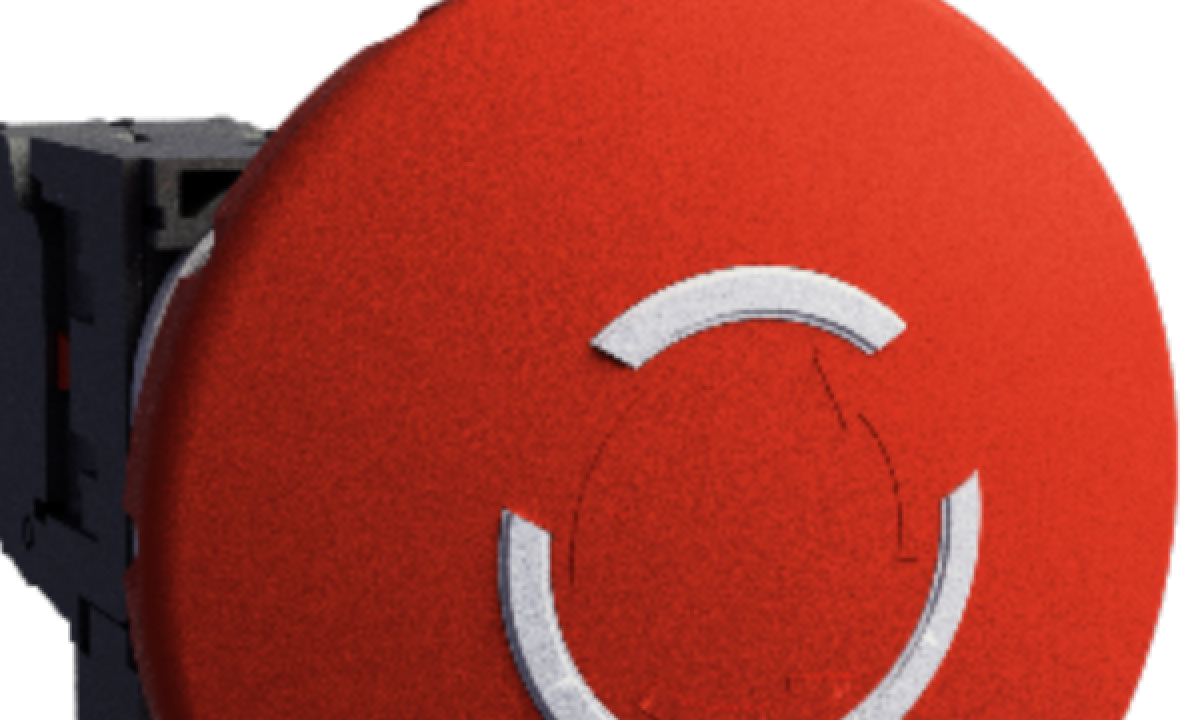
\includegraphics[width=\textwidth]{resources/denoise-off-100-samples.png}
        \caption{No denoising applied, 100 samples.}
        \label{fig:denoise-off}
    \end{subfigure}
    \hfill
    \begin{subfigure}[t]{0.38\textwidth}
        
\includegraphics[width=\textwidth]{resources/denoise-gaussian-100-samples.png}
        \caption{Denoise filtering applied, 100 samples.}
        \label{fig:denoise-gaussian-100-samples}
    \end{subfigure}
    \hspace*{0.8cm}
    \vfill
    \vspace*{0.5cm}
    \hspace*{0.8cm}
    \begin{subfigure}[t]{0.38\textwidth}
        
\includegraphics[width=\textwidth]{resources/denoise-oidn-100-samples.png}
        \caption{\gls{OIDN} applied, 100 samples.}
        \label{fig:denoise-oidn-100-samples}
    \end{subfigure}
    \hfill
    \begin{subfigure}[t]{0.38\textwidth}
        
\includegraphics[width=\textwidth]{resources/denoise-oidn-10-samples.png}
        \caption{\gls{OIDN} applied, 10 samples.}
        \label{fig:denoise-oidn-10-samples}
    \end{subfigure}
    \hspace*{0.8cm}
    \caption{Renderings with a limited number of samples demonstrating the effect of denoising.}
    \label{fig:denoise-samples}
\end{figure}

\newpage

\section{Documentation}

The path tracer is designed to be integrated into existing web projects. The package is installable via \gls{npm} but could also be downloaded and included manually. The complete documentation is available on the website. The documentation is designed to demonstrate the path tracer, provide a quick start guide, and offer detailed information on how to set up \texttt{strahl}. The website is shown in \autoref{fig:strahl-homepage}.

\begin{figure}[H]
    \centering
    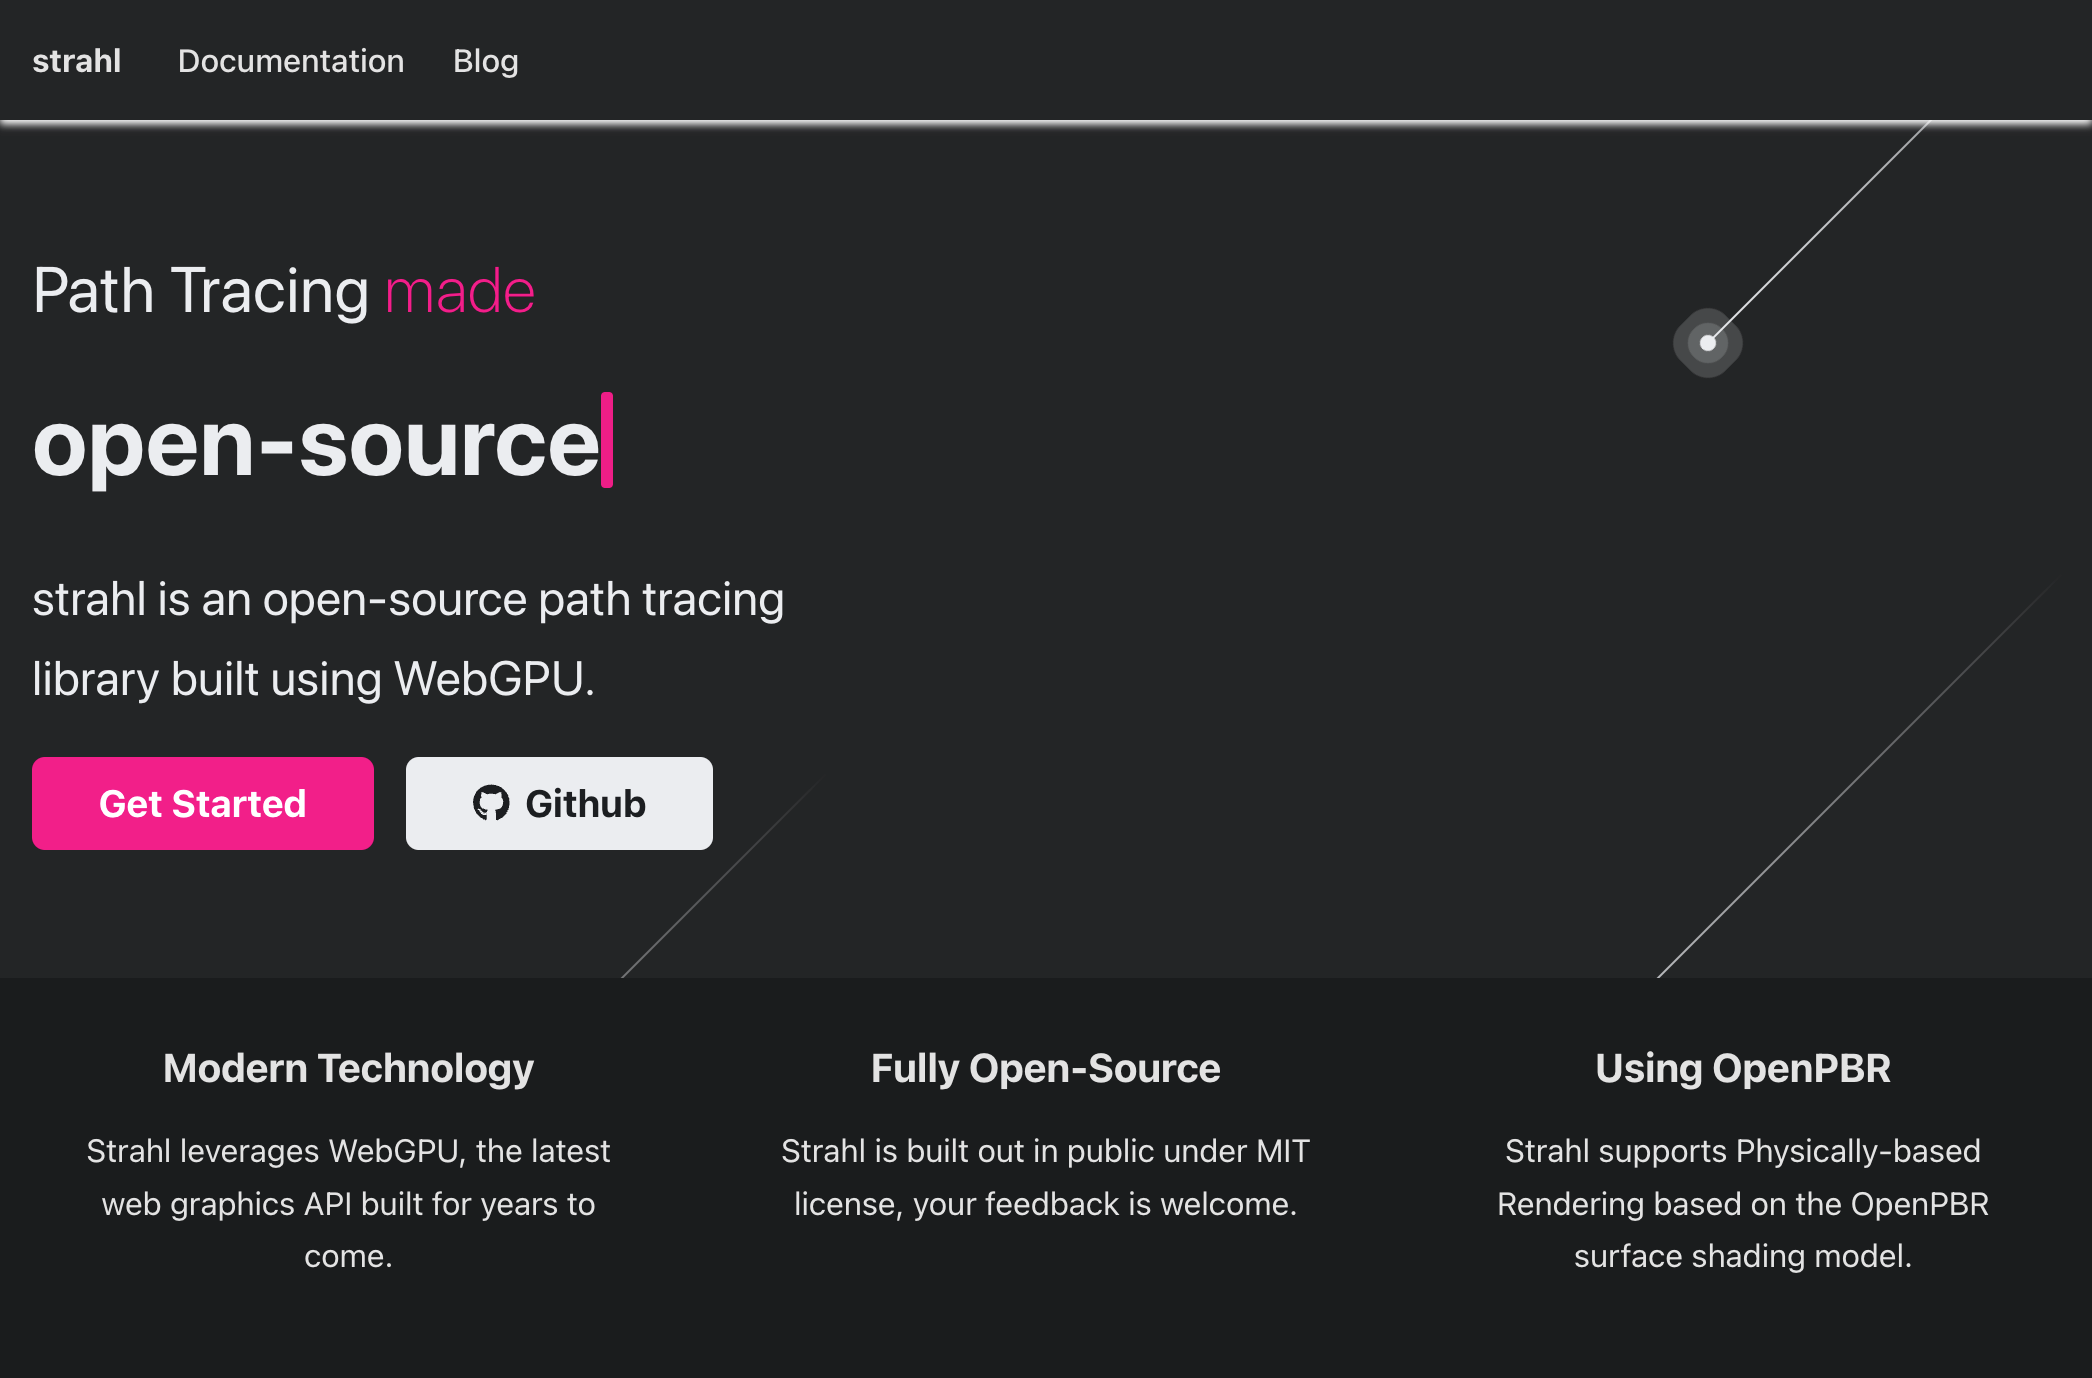
\includegraphics[width=0.95\columnwidth]{resources/website-home.png}
    \caption{Homepage of the \texttt{strahl} website.}
    \label{fig:strahl-homepage}
\end{figure}

Documentation on how to configure the renderer is provided. The library uses custom exceptions that the user can catch and handle. It provides different exceptions to enable the user to react appropriately to different error conditions. This includes basic exceptions where the action is limited, such as missing browser support for \gls{WebGPU}, as well as transparent information on what the user misconfigured. The use of \fGls{TypeScript}{a typed superset of JavaScript developed by Microsoft.} enables code completion and type checking. The documentation describes how to control sampling, denoising, environment lighting, and more. See \autoref{fig:strahl-documentation} for an example of a code snippet with an interactive sandbox.

\begin{figure}[H]
    \centering
    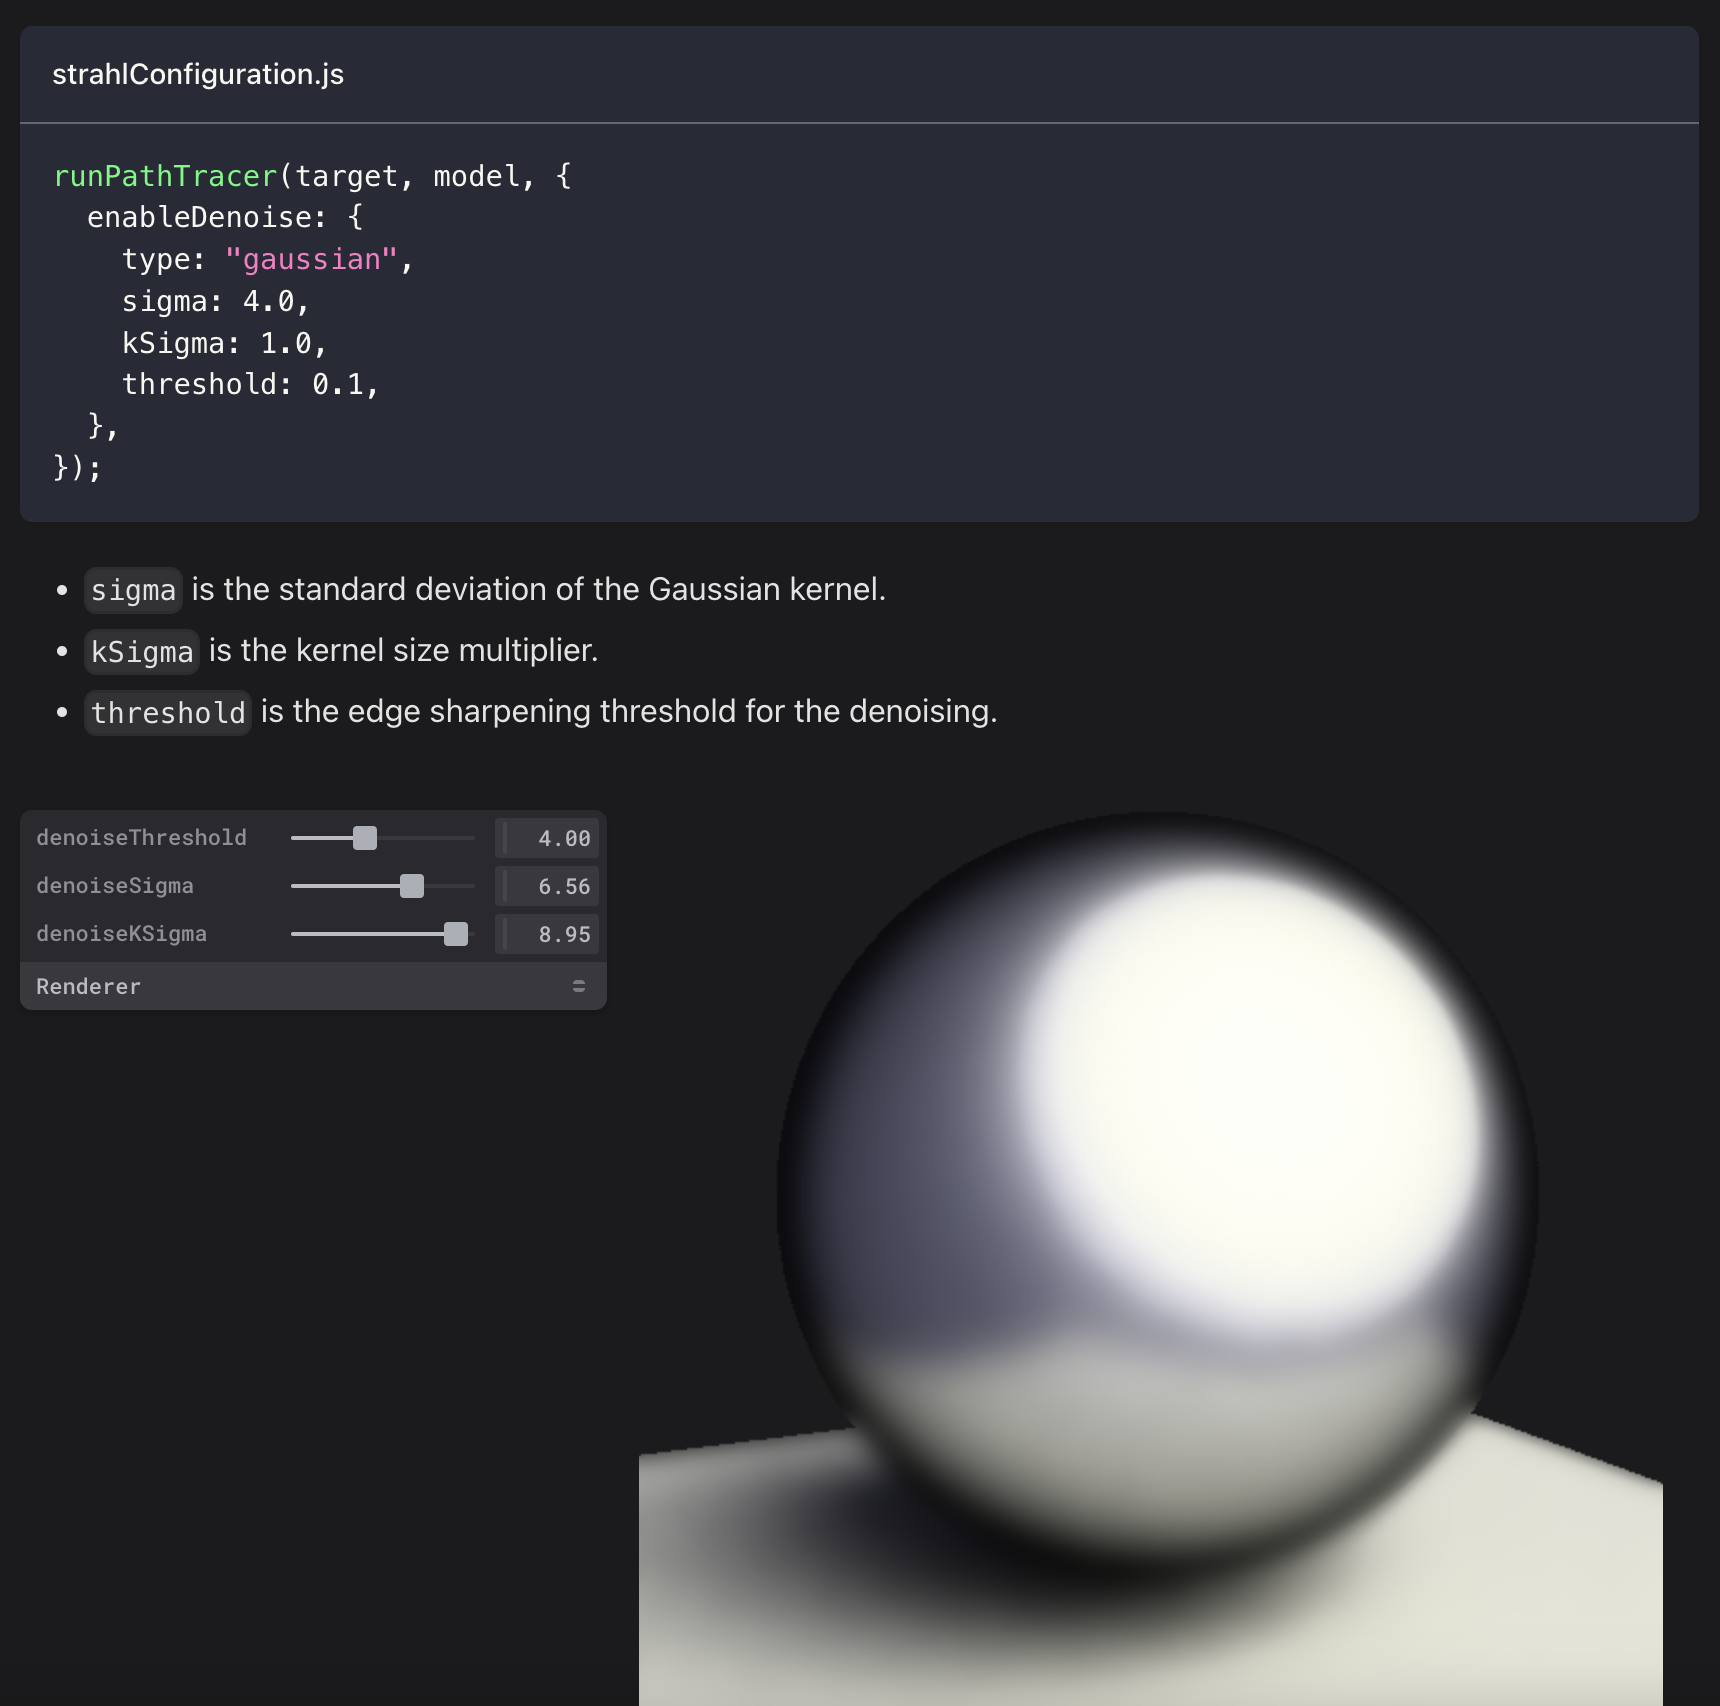
\includegraphics[width=0.7\columnwidth]{resources/website-documentation.png}
    \caption{Extract of documentation on how to set up denoising, with interactive sandbox.}
    \label{fig:strahl-documentation}
\end{figure}

The documentation includes showcases for the \gls{OpenPBR} surface shading model. The goal is to enable users to understand the parameter set and document how to configure materials to get the desired result. The parameters can be adjusted in real-time to see the effect on the rendering, as shown in \autoref{fig:docu-demo}.

\begin{figure}[H]
    \centering
    \begin{subfigure}[b]{0.45\textwidth}
        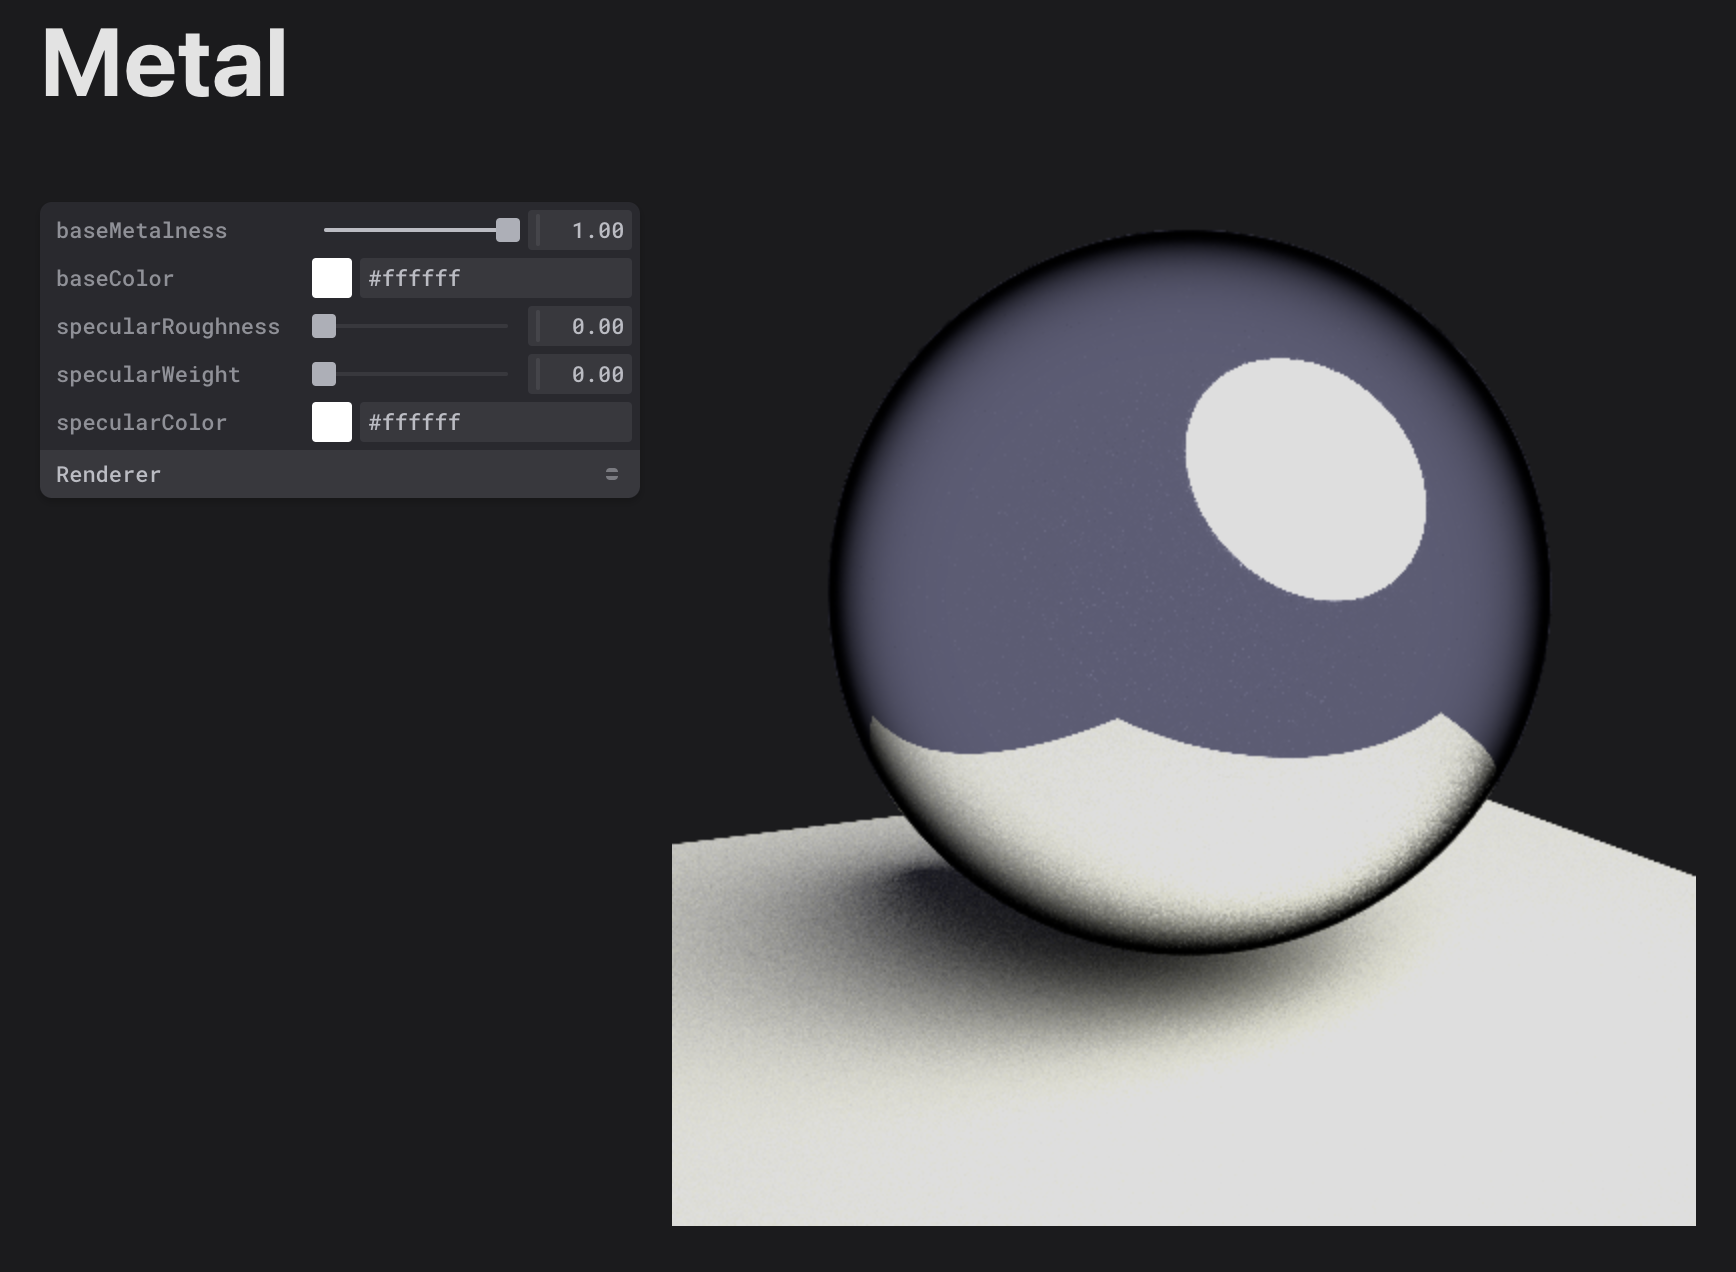
\includegraphics[width=\textwidth]{resources/docu-demo-mirror-metal.png}
        \caption{Mirror-like metal surface.}
        \label{fig:docu-demo-mirror}
    \end{subfigure}
    \hfill
    \begin{subfigure}[b]{0.45\textwidth}
        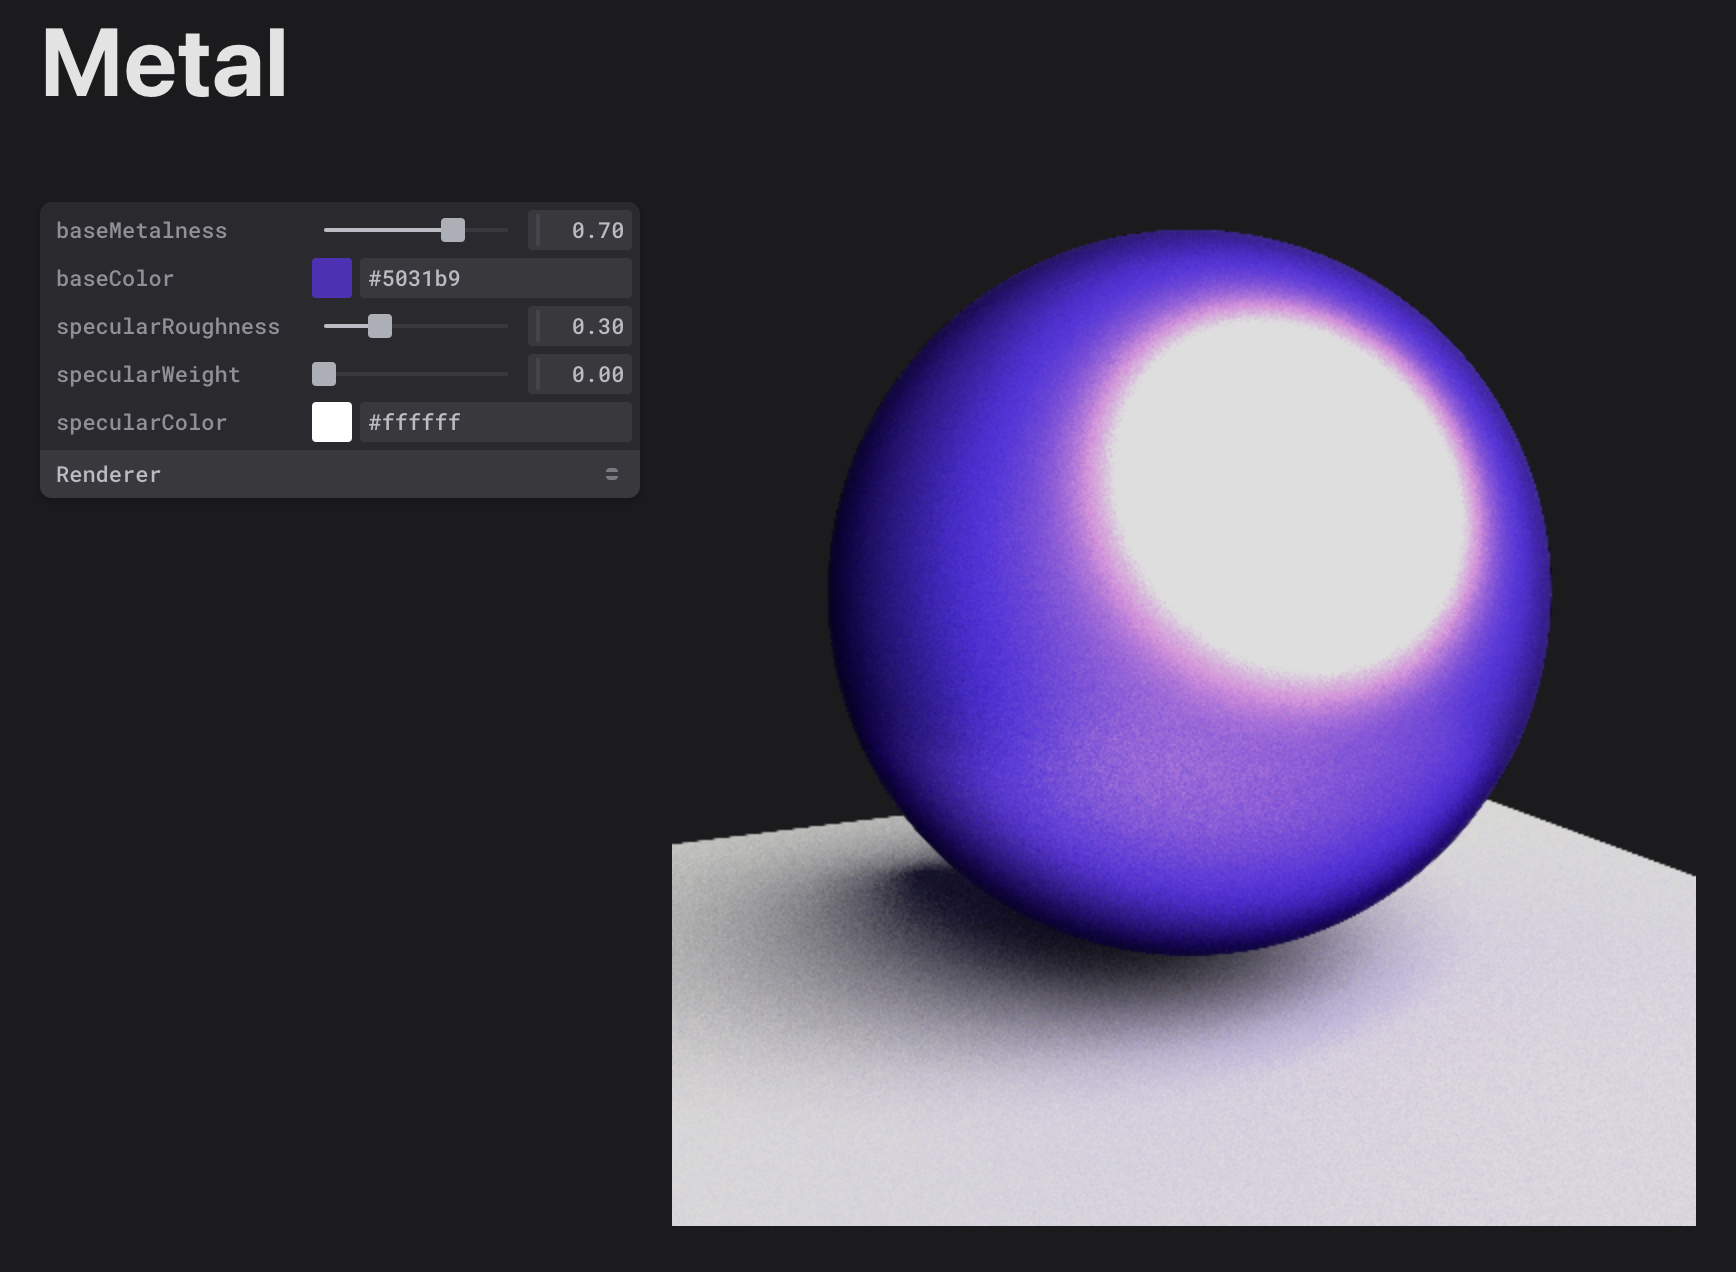
\includegraphics[width=\textwidth]{resources/docu-demo-rough-metal.png}
        \caption{Rougher metal surface.}
        \label{fig:docu-demo-rough}
    \end{subfigure}
    \caption{Configurable showcase for \gls{OpenPBR} parameters.}
    \label{fig:docu-demo}
\end{figure}

\section{Benchmark}
\label{sec:benchmark}

Prior sections, such as anti-aliasing, as described in \autoref{sec:anti-aliasing-implementation}, focus on qualitative aspects of the renderer. In order to assess the effectiveness of specific measures, a benchmark is defined to measure the performance of the path tracer. This benchmark is used for quantitative evaluation of the path tracer. The metrics can be adjusted depending on the use case. However, the core design of the benchmark remains the same. Generally, measurements are taken for the entirety of a stage instead of focusing on individual routines within a stage. This gives a more holistic view of the performance of the path tracer. The results focus on \gls{GPU} performance. The measurements are recorded using two systems. The first is based on \gls{WebGPU} timestamp queries that only account for the compute pipeline. The second is taking wall-clock time using the Performance \gls{API} for the entire \gls{GPU} part. The results presented are based on wall-clock time.

A total of 100 samples per pixel with a ray depth of five is used. The image is rendered in Chrome 127/128 at a resolution of 512$\times$512 pixels. Experiments are conducted with different model complexities. The simplified versions are decimated meshes of the original, which consists of roughly one million triangles. The \gls{LOD} artifacts can be seen in \autoref{fig:benchmark-models}. The first two levels are intended to be visually similar, while the third level is a simplified version intended to demonstrate the effect of non-manifold geometry for ray tracing.

Unless otherwise specified, the benchmarks are conducted on a MacBook Pro with Apple Silicon M1 Max. The measurements are calculated using the mean time of 30 runs with a confidence interval of 95\% given as $\pm$ standard deviation from the mean time in milliseconds (ms) as described in \autoref{sec:probabilityTheory}. The different measurement sections should not be compared directly, as different factors influence them and may have been taken at different development stages of the renderer. They are only intended for comparison within the same measurement category.

\begin{figure}[H]
    \centering
    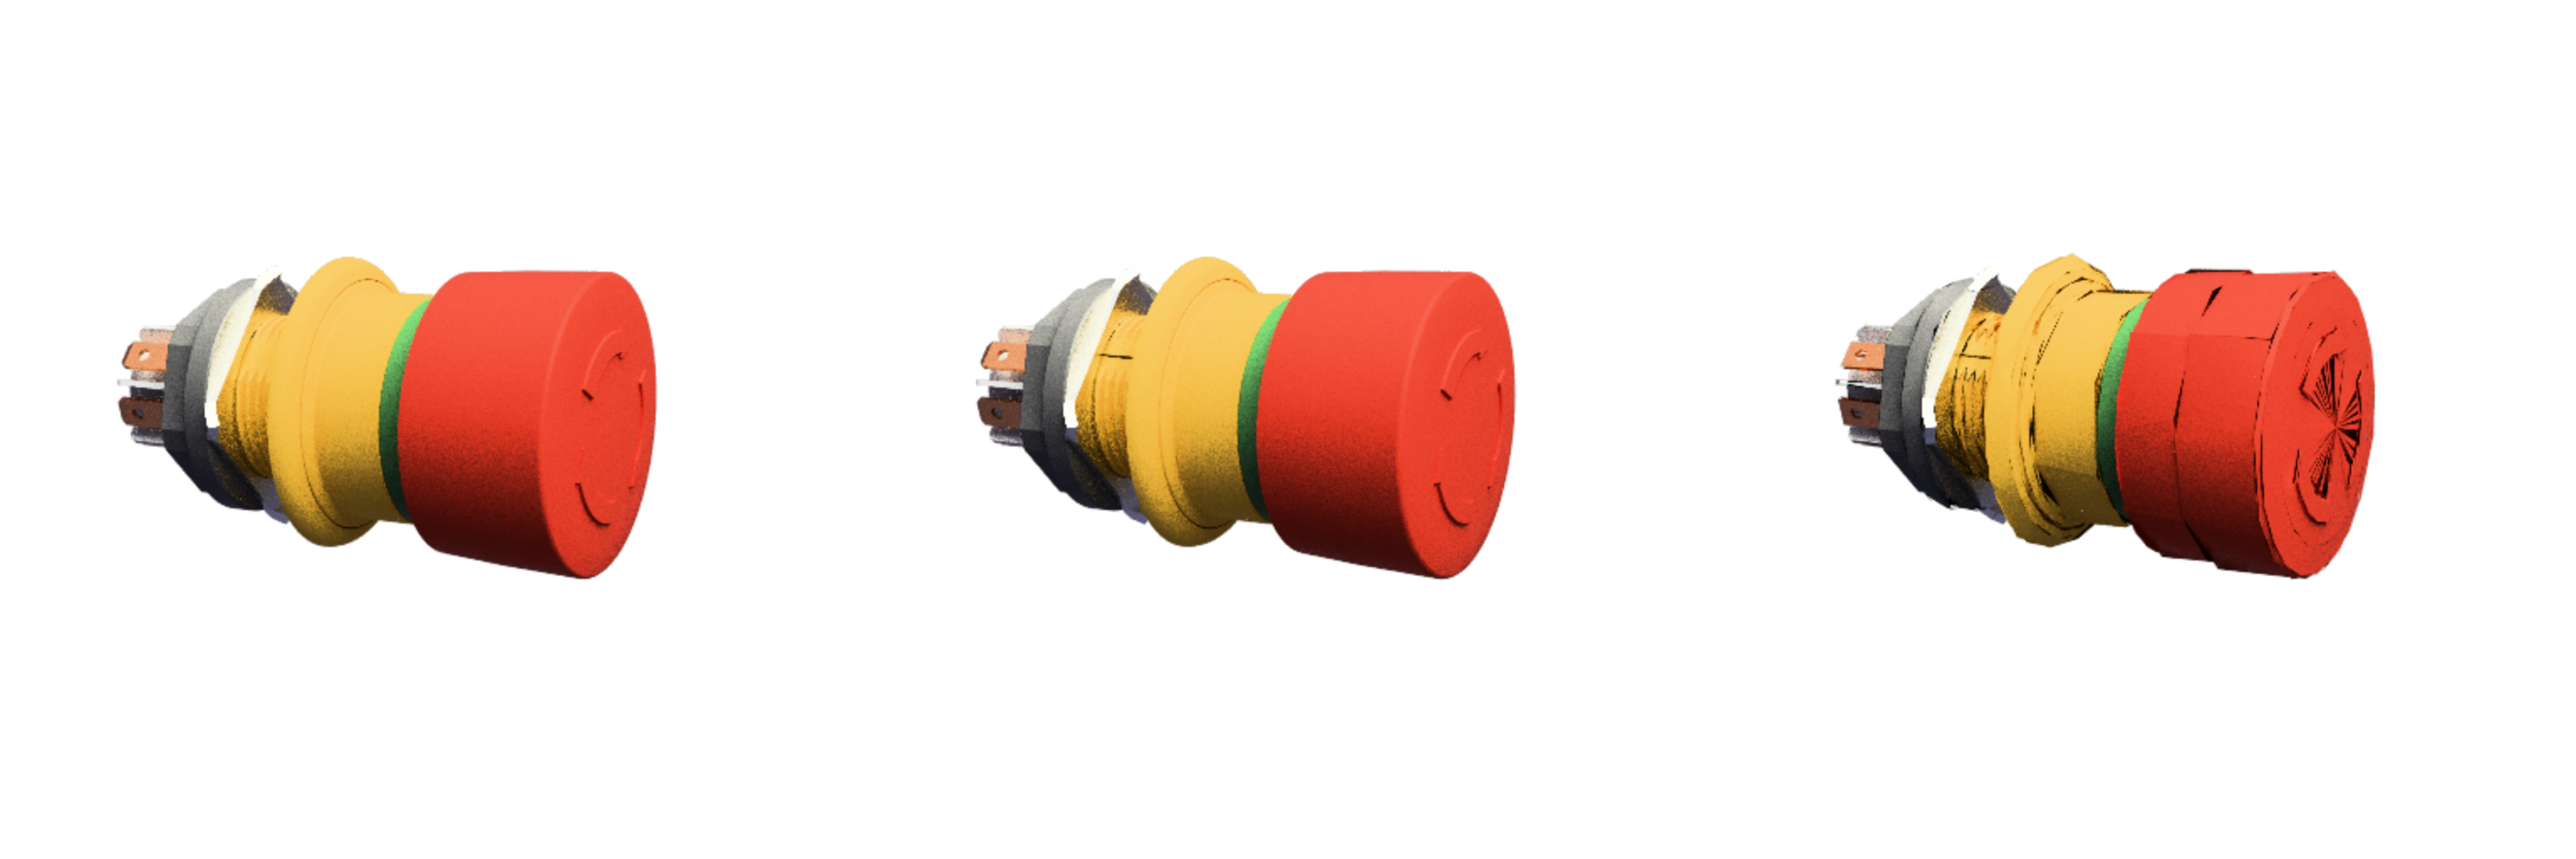
\includegraphics[width=0.9\columnwidth]{resources/benchmark-models.png}
    \caption{The three \gls{LOD} artifacts and their short names in brackets, from left to right: 1,068,735 triangles (high), 106,873 triangles (mid), and 10,687 triangles (low). The left and middle figures share similar visual fidelity characteristics.}
    \label{fig:benchmark-models}
\end{figure}

\subsection*{Russian Roulette}

As described in \autoref{ch:russianRoulette}, Russian roulette is a technique for probabilistic path termination. The code is implemented in \coderef{RUSSIAN-ROULETTE}. The benchmark results for the path tracing routine are shown in \autoref{tab:russian-roulette-measurements}.

\begin{table}[H]
    \centering
    \ra{1.3}
    \begin{tabular}{@{}lrr@{}}
        \toprule
             & With Russian roulette      & Without Russian roulette   \\
        High & 2,361.77 ms $\pm$ 11.27 ms & 2,583.40 ms $\pm$ 12.84 ms \\
        Mid  & 2,018.03 ms $\pm$ 8.76 ms  & 2,135.94 ms $\pm$ 8.14 ms  \\
        Low  & 2,028.04 ms $\pm$ 10.78 ms & 2,200.00 ms $\pm$ 8.91 ms  \\
        \bottomrule
    \end{tabular}
    \caption{Benchmark results for Russian roulette optimization.}
    \label{tab:russian-roulette-measurements}
\end{table}

\subsection*{BVH Split Axis Heuristic}

For the intersection tests using the \gls{BVH}, the split axis is used as a heuristic for node traversal, as described in \autoref{sec:bvh-implementation}. In order to assess the effectiveness of the heuristic, the benchmark results for the path tracing routine are shown in \autoref{tab:bvh-split-axis-measurements}.

\begin{table}[H]
    \centering
    \ra{1.3}
    \begin{tabular}{@{}lrr@{}}
        \toprule
             & With split axis heuristic  & Without split axis heuristic \\
        High & 3,244.30 ms $\pm$ 45.71 ms & 4,039.87 ms $\pm$ 33.51 ms   \\
        Mid  & 2,663.14 ms $\pm$ 35.57 ms & 3,181.89 ms $\pm$ 24.92 ms   \\
        Low  & 2,698.65 ms $\pm$ 27.60 ms & 3,124.27 ms $\pm$ 36.02 ms   \\
        \bottomrule
    \end{tabular}
    \caption{Benchmark results for \gls{BVH} split axis heuristic.}
    \label{tab:bvh-split-axis-measurements}
\end{table}

\subsection*{Sampling Time Comparison}

The time for each individual sample remains consistent across benchmark runs. This means that sample \#1 will take a similar amount of time during all runs. However, the time of different samples within the same run is inconsistent. Primarily, the first sample takes substantially longer than the rest of the samples, as can be seen in \autoref{dia:sampling-times}. The average time for sample \#2 is 27.53~ms $\pm$ 1.38~ms, whereas sample \#1 takes 102.83~ms $\pm$ 1.26~ms. These measurements were collected using the high \gls{LOD} artifact. After the \gls{CPU} preparation and \gls{GPU} preheating, which consists of the first sample, the path tracer can render approximately 35 samples per second.

\begin{figure}
    \centering
    \tikzsetnextfilename{sampling-times}
    \begin{tikzpicture}
        \begin{axis}[
                width=14cm,
                height=6.5cm,
                xlabel={Sample Number},
                ylabel={Render Time (ms)},
                ylabel near ticks,
                symbolic x coords={\#1,\#2,\#3,\#4,\#5,\#6,\#7,\#8,\#9,\#10},
                xtick=data,
                ytick={30, 60, 100},
                ymin=0,
                ymax=110,
                ymajorgrids=true,
                grid style=dashed,
            ]
            \addplot[
                ybar,
                fill=rbblue,
                draw=rblue,
                thick,
                error bars/.cd,
                y dir=both,
                y explicit
            ]
            coordinates {
                    (\#1,102.83) +- (0,1.26)
                    (\#2,27.53) +- (0,1.38)
                    (\#3,26.94) +- (0,1.11)
                    (\#4,26.41) +- (0,1.29)
                    (\#5,26.96) +- (0,1.25)
                    (\#6,26.19) +- (0,1.13)
                    (\#7,26.41) +- (0,1.09)
                    (\#8,26.08) +- (0,1.27)
                    (\#9,25.97) +- (0,0.82)
                    (\#10,26.64) +- (0,1.10)
                };
        \end{axis}
    \end{tikzpicture}
    \caption{Mean time per sample, showing that the first sample consistently takes longer than subsequent samples. The chart is limited to ten samples as the results for the remaining samples are similar to samples \#2 until \#10.}
    \label{dia:sampling-times}
\end{figure}

\newpage
\subsection*{Overall Performance}

A final performance test was conducted on two machines. The AMD/NVIDIA machine is a desktop computer with an AMD Ryzen~5 5600X \gls{CPU} and NVIDIA GeForce RTX~3080 (10 GB) \gls{GPU}. The \gls{CPU} results for setting up the \gls{BVH} are measured using the Performance \gls{API} and can be seen in \autoref{tab:cpuPerformance}. The \gls{GPU} results for the core path tracing are presented in \autoref{tab:gpuPerformance}.

\begin{table}[H]
    \centering
    \ra{1.3}
    \begin{tabular}{lrr}
        \toprule
             & Apple M1 Max            & AMD/NVIDIA              \\
        High & 351.87 ms $\pm$ 1.04 ms & 366.33 ms $\pm$ 1.10 ms \\
        Mid  & 47.63 ms $\pm$ 0.33 ms  & 46.43 ms $\pm$ 1.10 ms  \\
        Low  & 9.79 ms $\pm$ 0.07 ms   & 10.03 ms $\pm$ 0.25 ms  \\
        \bottomrule
    \end{tabular}
    \caption{\gls{BVH} setup time based on model complexity.}
    \label{tab:cpuPerformance}
\end{table}

\begin{table}[H]
    \centering
    \ra{1.3}
    \begin{tabular}{lrr}
        \toprule
             & Apple M1 Max               & AMD/NVIDIA                  \\
        High & 2,693.78 ms $\pm$ 14.96 ms & 1,398.57 ms $\pm$ 131.38 ms \\
        Mid  & 2,315.97 ms $\pm$ 27.52 ms & 1,071.33 ms $\pm$ 83.74 ms  \\
        Low  & 2,387.14 ms $\pm$ 26.56 ms & 1,126.50 ms $\pm$ 73.92 ms  \\
        \bottomrule
    \end{tabular}
    \caption{\gls{GPU} path tracer time based on model complexity.}
    \label{tab:gpuPerformance}
\end{table}

\newpage
\section{Use Case Scenarios}

Different configurations based on engineering \gls{CAD} data used by EAO as rendered by the path tracer can be seen in \autoref{fig:rendering-showcase}. Note that artistic liberties were taken to highlight specific effects. The path tracer can render full configurations without being impeded by the complexity of the geometry. The renderer offers flexibility by providing configuration of \gls{OpenPBR} parameters, environment lighting, denoising setup, and more. The required number of samples is dependent on the scene. Effects such as rough metallic reflection require more samples to converge than a diffuse surface. For many use cases, the number is in the range of 100 to 1,000 samples per pixel. The library enables the user to obtain high-fidelity renderings of \gls{CAD} data without the need for pregenerated artifacts.

\begin{figure}[H]
    \centering
    \hspace*{0.6cm}
    \begin{subfigure}[t]{0.4\textwidth}
        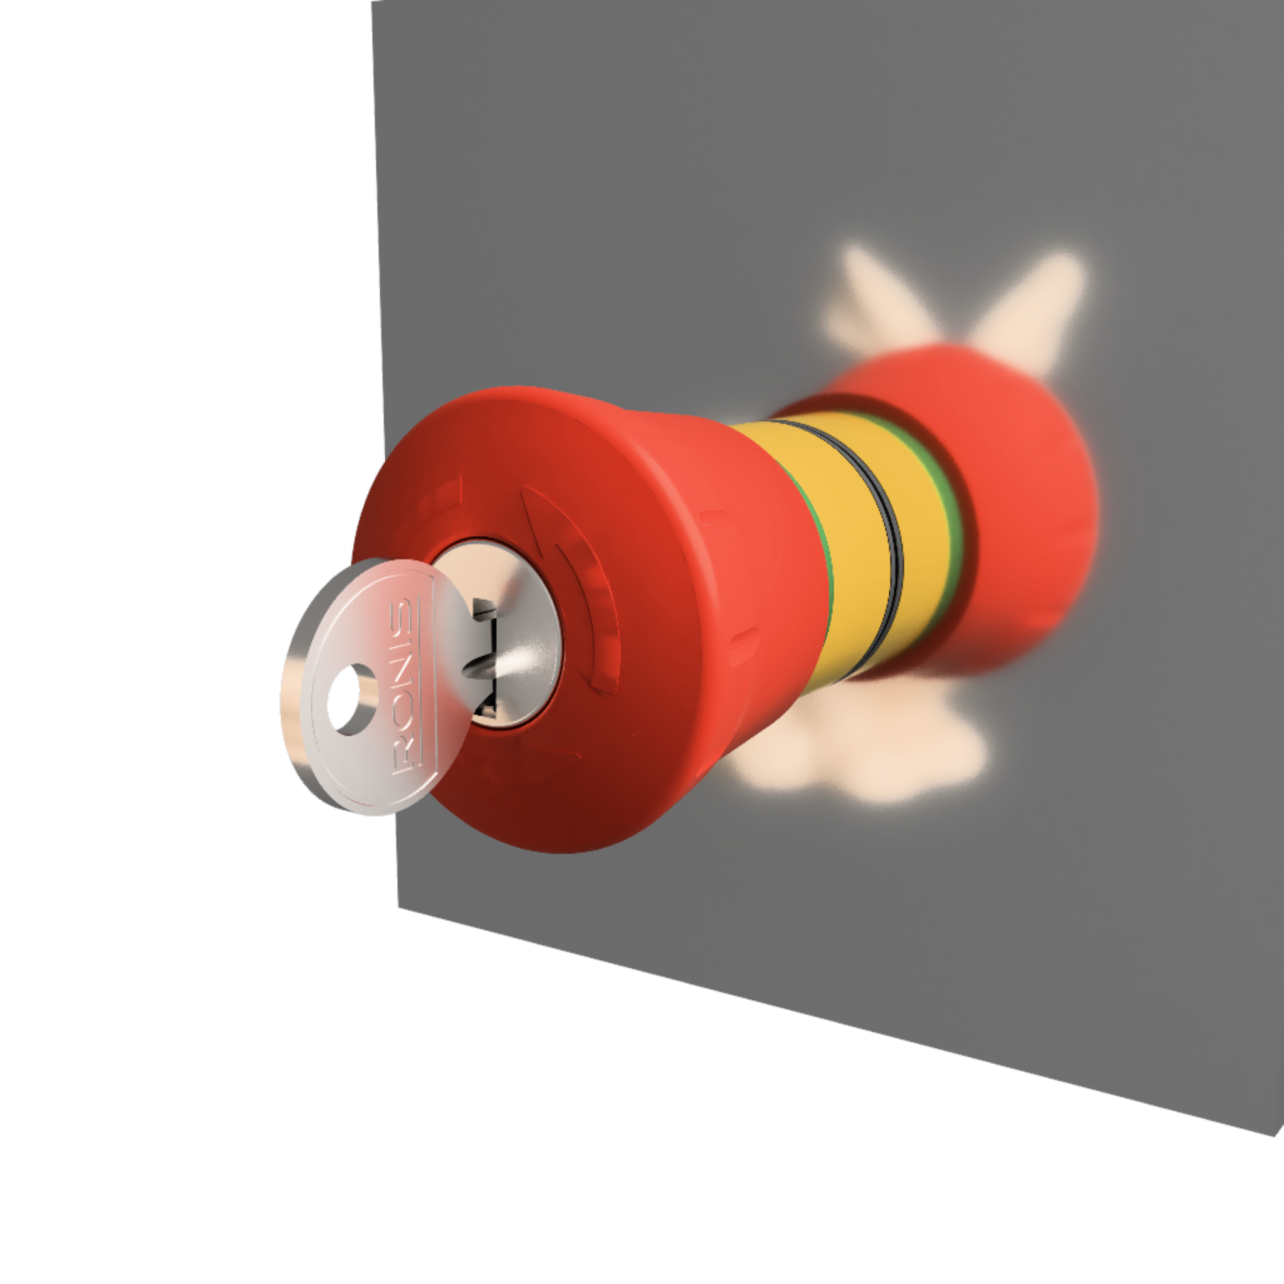
\includegraphics[width=\textwidth]{resources/demo-reflection.png}
        \caption{Pushbutton mounted on a metallic surface, including the reflection of the Stanford bunny model \cite{turkLevoy1994} positioned in the scene.}
        \label{fig:demo-reflection}
    \end{subfigure}
    \hfill
    \begin{subfigure}[t]{0.4\textwidth}
        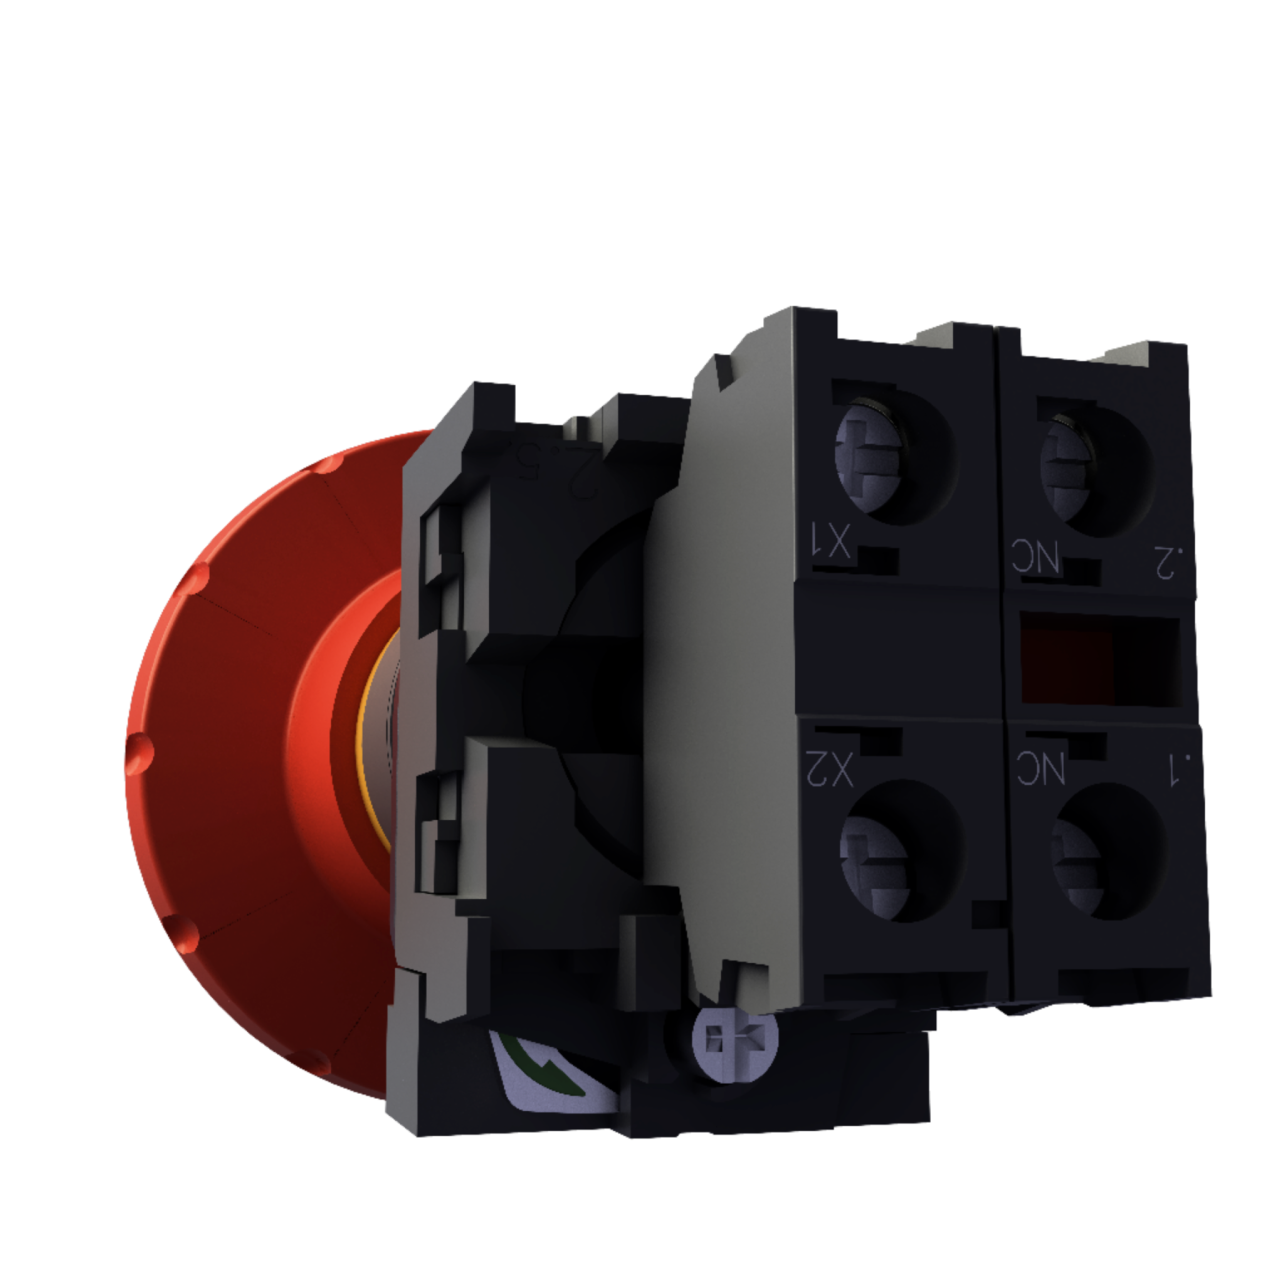
\includegraphics[width=\textwidth]{resources/demo-color-bleeding.png}
        \caption{Rear view exhibiting slight color bleeding, visible as a red tint on the black surface.}
        \label{fig:demo-color-bleeding}
    \end{subfigure}
    \hspace*{0.6cm}
    \vfill
    \vspace*{0.5cm}
    \hspace*{0.6cm}
    \begin{subfigure}[t]{0.4\textwidth}
        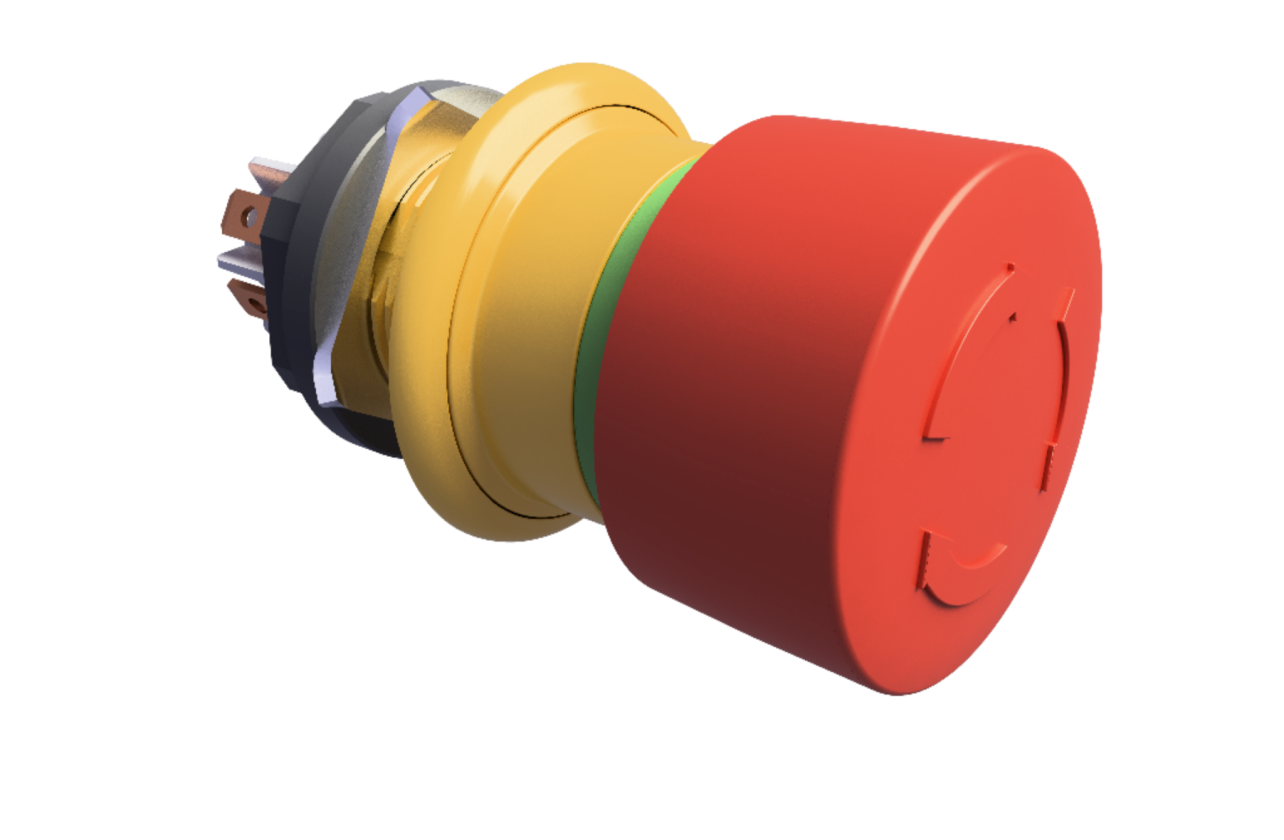
\includegraphics[width=\textwidth]{resources/demo-specular.png}
        \caption{Front view of pushbutton with specular highlights.}
        \label{fig:demo-specular}
    \end{subfigure}
    \hfill
    \begin{subfigure}[t]{0.4\textwidth}
        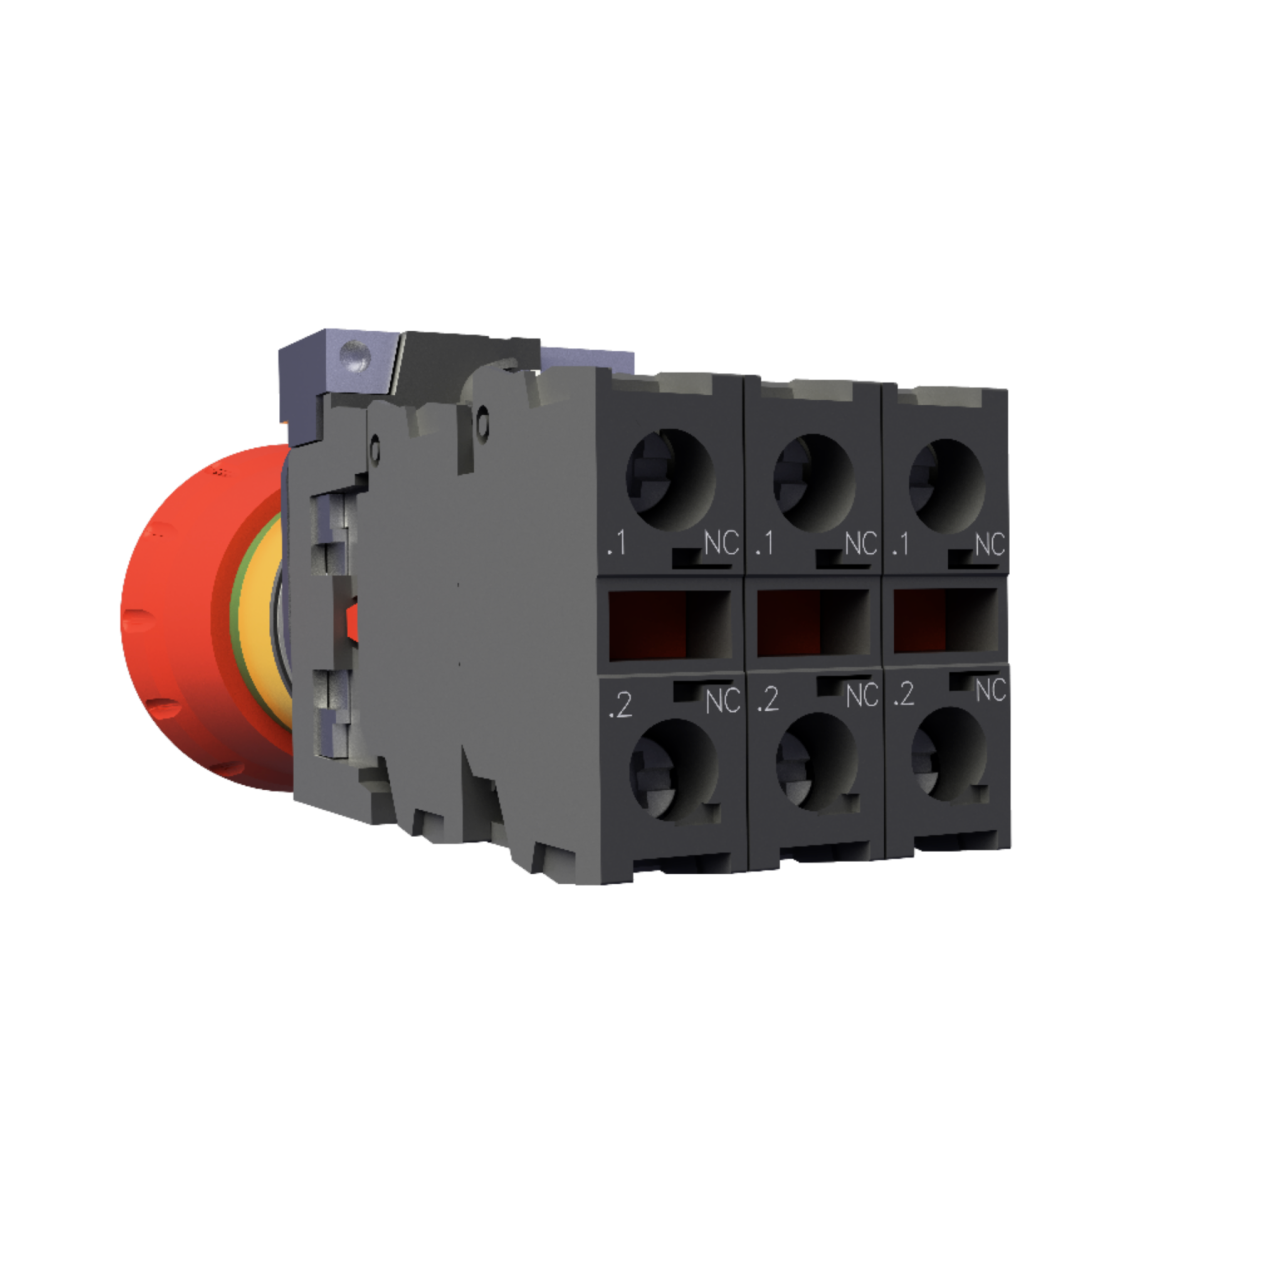
\includegraphics[width=\textwidth]{resources/demo-ambient-occlusion.png}
        \caption{Rear view demonstrating ambient occlusion.}
        \label{fig:demo-ambient-occlusion}
    \end{subfigure}
    \hspace*{0.6cm}
    \caption{Path-traced renderings of pushbutton \gls{CAD} models.}
    \label{fig:rendering-showcase}
\end{figure}
